%% =====================================================================
%% PEARL -- version restructured for submission to
%% Machine Intelligence Research (MIR), Springer Nature.
%%
%% IMPORTANT TEMPLATE NOTE (read before submitting):
%% I could not access MIR's authenticated "Submission guidelines" page
%% (link.springer.com/journal/11633/submission-guidelines redirects to a
%% Springer login wall), so the exact required \documentclass, class
%% options, and .bst reference style for MIR could NOT be verified.
%% This file therefore uses a safe, universally-compiling base (standard
%% `article` class + common packages) so it compiles as-is. Before
%% submission:
%%   1. Download the official Springer Nature LaTeX template from
%%      https://www.springernature.com/gp/authors/campaigns/latex-author-support
%%      (this is the confirmed source for MIR's template family).
%%   2. Replace the preamble below (\documentclass...\begin{document}
%%      through \maketitle) with that template's title-page macros.
%%   3. Replace \bibliographystyle{unsrt} with MIR's required style file
%%      (shipped inside the Springer Nature template bundle).
%% All article CONTENT below (text, tables, figures, citations, numbers)
%% is otherwise unchanged from the verified main manuscript.
%% =====================================================================

\documentclass[11pt]{article}

\usepackage[margin=1in]{geometry}
\usepackage{amssymb}
\usepackage{amsmath}
\usepackage{graphicx}
\usepackage{url}
\usepackage{adjustbox}
\usepackage{booktabs}
\usepackage{authblk}

\title{PEARL: A Parameter-Efficient Retrieval-Augmented Benchmarking Framework for Molecular Property Prediction}

\author[1]{Kavya Agarwal}
\author[1]{Sukrit Gupta}
\author[2]{Halima Bensmail}
\author[2,3]{Raghvendra Mall\thanks{Corresponding author: ramall@hbku.edu.qa, raghvendramall@ieee.org}}

\affil[1]{Center for Applied Research in Data Science, Indian Institute of Technology Ropar, Rupnagar, Punjab 140001, India}
\affil[2]{Qatar Computing Research Institute, Hamad Bin Khalifa University, Doha, Qatar}
\affil[3]{Translational Medicine Department, Sidra Medicine, Doha, Qatar}

\date{}

\begin{document}
\maketitle

\begin{abstract}
\noindent
Molecular property prediction sits at the center of computational drug discovery, and it hinges on a tension between two complementary views of a molecule: the sequential chemistry encoded in a SMILES string and the three-dimensional geometry that actually governs binding and toxicity. Standard full-finetuning of chemical language models (CLMs) that capture the former is computationally heavy, and 1D SMILES-based models have no explicit inductive bias for the latter -- yet no benchmark has directly compared parameter-efficient adaptation of 1D CLMs against a SE(3)-equivariant 3D model across diverse tasks and adaptation regimes (classification \emph{and} regression), while also controlling for a strong, non-CLM baseline. We introduce \textbf{PEARL} (\textbf{P}arameter-\textbf{E}fficient \textbf{A}daptation with \textbf{R}etrieval-augmented \textbf{L}earning), which combines Low-Rank Adaptation (LoRA) uniformly across three CLM families -- ChemBERTa, MolFormer, and Uni-Mol -- with a Retrieval-Augmented Feature Enhancement (RAFE) pipeline that enriches predictions with label-free physicochemical neighborhood context retrieved from the ZINC-250k knowledge base, and benchmarks both against in-house Chemprop, GCN, and PC-only (no-CLM) baselines run under an identical protocol on seven molecular property datasets. Uni-Mol's SE(3)-equivariant architecture achieves the best BACE inhibitor classification (MCC$=0.623$), an $8\%$ absolute gain over the best SMILES-based model, confirming that 3D geometry provides an inductive advantage where binding affinity is mechanistically 3D; RAFE is the point-estimate winner on BBBP (MCC$=0.798$) and DILI (MCC$=0.790$), narrowing but not fully closing the gap to explicit 3D structure elsewhere. LoRA reduces trainable parameters by $76$--$97\%$ across all three CLM families with no accuracy loss, though a strong, non-neural PC-only baseline remains statistically competitive on five of the seven datasets, indicating that CLM complexity does not always pay for itself. Code, data-curation pipelines, and all baseline implementations are open-sourced at \url{https://github.com/raghvendra5688/PEARL}.
\end{abstract}

\noindent\textbf{Keywords:} Retrieval-Augmented Generation, Parameter-Efficient Finetuning, Chemical Language Models, Low-Rank Adaptation, 3D Molecular Representations, ADMET Property Prediction, Computational Drug Discovery, Chemoinformatics

%% =====================================================================
\section{Introduction}\label{sec:intro}

Understanding how molecular structure determines biological or physicochemical properties sits at the heart of computational drug discovery. Traditional quantitative structure-activity relationship (QSAR) methods lean on handcrafted molecular descriptors, but deep learning, and transformer-based architectures~\cite{vaswani2017attention} in particular, now let us learn molecular representations end-to-end directly from a molecule's Simplified Molecular Input Line Entry System (SMILES) sequence. That shift has driven the rise of chemical language models (CLMs) pretrained on enormous molecular corpora, which increasingly rival experimental approaches for predicting toxicity, solubility, and bioactivity~\cite{ahmad2022chemberta2,huang2020deeppurpose}.

Three problems, though, keep coming up. First, CLMs treat SMILES as flat token sequences, so they have no built-in notion of the three-dimensional geometry that governs binding affinity and enzyme inhibition. Second, fine-tuning an $\mathcal{O}(10^8)$-parameter CLM separately for each specialized task is often simply too expensive in resource-constrained settings. Third, and perhaps most avoidably, CLM benchmarking papers routinely compare against GNN baselines \emph{cited from other papers} rather than re-run under the same splits, preprocessing, and evaluation protocol, which makes a reported ``win'' hard to interpret causally.

Here we take on all three at once. We work with three model families: MolFormer~\cite{ross2022molformer}, ChemBERTa-2~\cite{ahmad2022chemberta2}, and Uni-Mol~\cite{zhou2023unimol}, the last a SE(3)-equivariant Transformer that operates directly on explicit 3D atomic coordinates, and apply Low-Rank Adaptation (LoRA)~\cite{hu2021lora} to each. On top of this we build a \emph{Retrieval-Augmented Feature Enhancement} (RAFE) framework, which uses task-specific finetuned embeddings to pull the nearest chemical neighbors from ZINC-250k~\cite{gomez2018automatic}, a 249,455-molecule drug-like library, via GPU-accelerated FAISS indices~\cite{johnson2021faiss}. And to close the third gap, for every one of the seven datasets we train Chemprop~\cite{yang2019chemprop} and a graph convolutional network (GCN) \emph{in-house}, under the same scaffold split and bootstrapped-CI evaluation protocol as every CLM-based method. Alongside these we add a \textbf{PC-only} baseline: a tree ensemble trained purely on 473 engineered physicochemical (PC) descriptors, with no CLM embedding at all. That baseline suite is what lets us actually answer whether the CLM ladder (End-to-End [E2E] LoRA, Finetune [FT] Embed, FT Embed+PC, RAFE) earns its added complexity over a much simpler, non-neural alternative.

We benchmark PEARL on seven molecular property prediction datasets: three MoleculeNet-era classification tasks, namely $\beta$-secretase inhibition (BACE), blood-brain-barrier prediction (BBBP), and flavor (Flavor) prediction. The other four come from the Therapeutics Data Commons (TDC) ADMET Group~\cite{huang2021tdc}: hERG cardiac-channel inhibition~\cite{wang2016herg}, drug-induced liver injury (DILI)~\cite{xu2019dili}, Caco-2 permeability (regression)~\cite{wang2016caco2}, and drug half-life (regression)~\cite{obach2008half}. Two of the seven are regression tasks, which means the PEARL ladder, RAFE, and every baseline all need to support Huber-loss finetuning and R\textsuperscript{2}/MAE/Spearman evaluation, described in Section~\ref{sec:pearl_arch}.

Our core contributions are:
\begin{itemize}
  \item \textbf{The PEARL framework}, which unifies parameter-efficient LoRA adaptation across three CLM families (ChemBERTa, MolFormer, Uni-Mol) with a novel Retrieval-Augmented Feature Enhancement (RAFE) pipeline that injects label-free physicochemical neighborhood context from an external knowledge base (ZINC-250k), spanning classification and regression targets alike.
  \item \textbf{A systematic, uniform benchmark} across all three CLM families and both 1D/3D representations, using seven molecular property datasets and an identical scaffold split, hyperparameter search budget, and bootstrapped-CI evaluation protocol for every method, including in-house-retrained Chemprop, GCN, and PC-only baselines rather than numbers cited from other papers.
  \item \textbf{Insights into whether retrieval augmentation substitutes for explicit 3D geometry}: RAFE is the overall point-estimate winner on BBBP (MCC$=0.798$) and DILI (MCC$=0.790$), but only Uni-Mol's explicit 3D SE(3)-equivariant architecture clears the PC-only baseline by a statistically confirmed margin on BACE (MCC$=0.623$), indicating that label-free retrieval features narrow, without fully closing, the gap to explicit 3D structural information on tasks where binding geometry is mechanistically decisive.
  \item All code, including the TDC data-curation, RAFE, and in-house GNN baseline pipelines, is publicly available at \url{https://github.com/raghvendra5688/PEARL}.
\end{itemize}

Figure~\ref{fig:workflow} illustrates the complete PEARL workflow. The molecular dataset is processed by one of three CLM backbones. LoRA adapters augment only the attention projection layers, keeping all other pretrained weights frozen. For Uni-Mol, 3D conformers (SE(3)) are pre-generated via ETKDGv3 + MMFF94 and cached. The finetuned model provides both end-to-end predictions and task-specific embeddings. These embeddings are optionally concatenated with engineered PC features and with ZINC-250k RAFE features retrieved via FAISS indices, and the resulting feature vector is fed to Optuna-tuned tree-based classifiers or regressors.

\begin{figure*}[!ht]
  \centering
  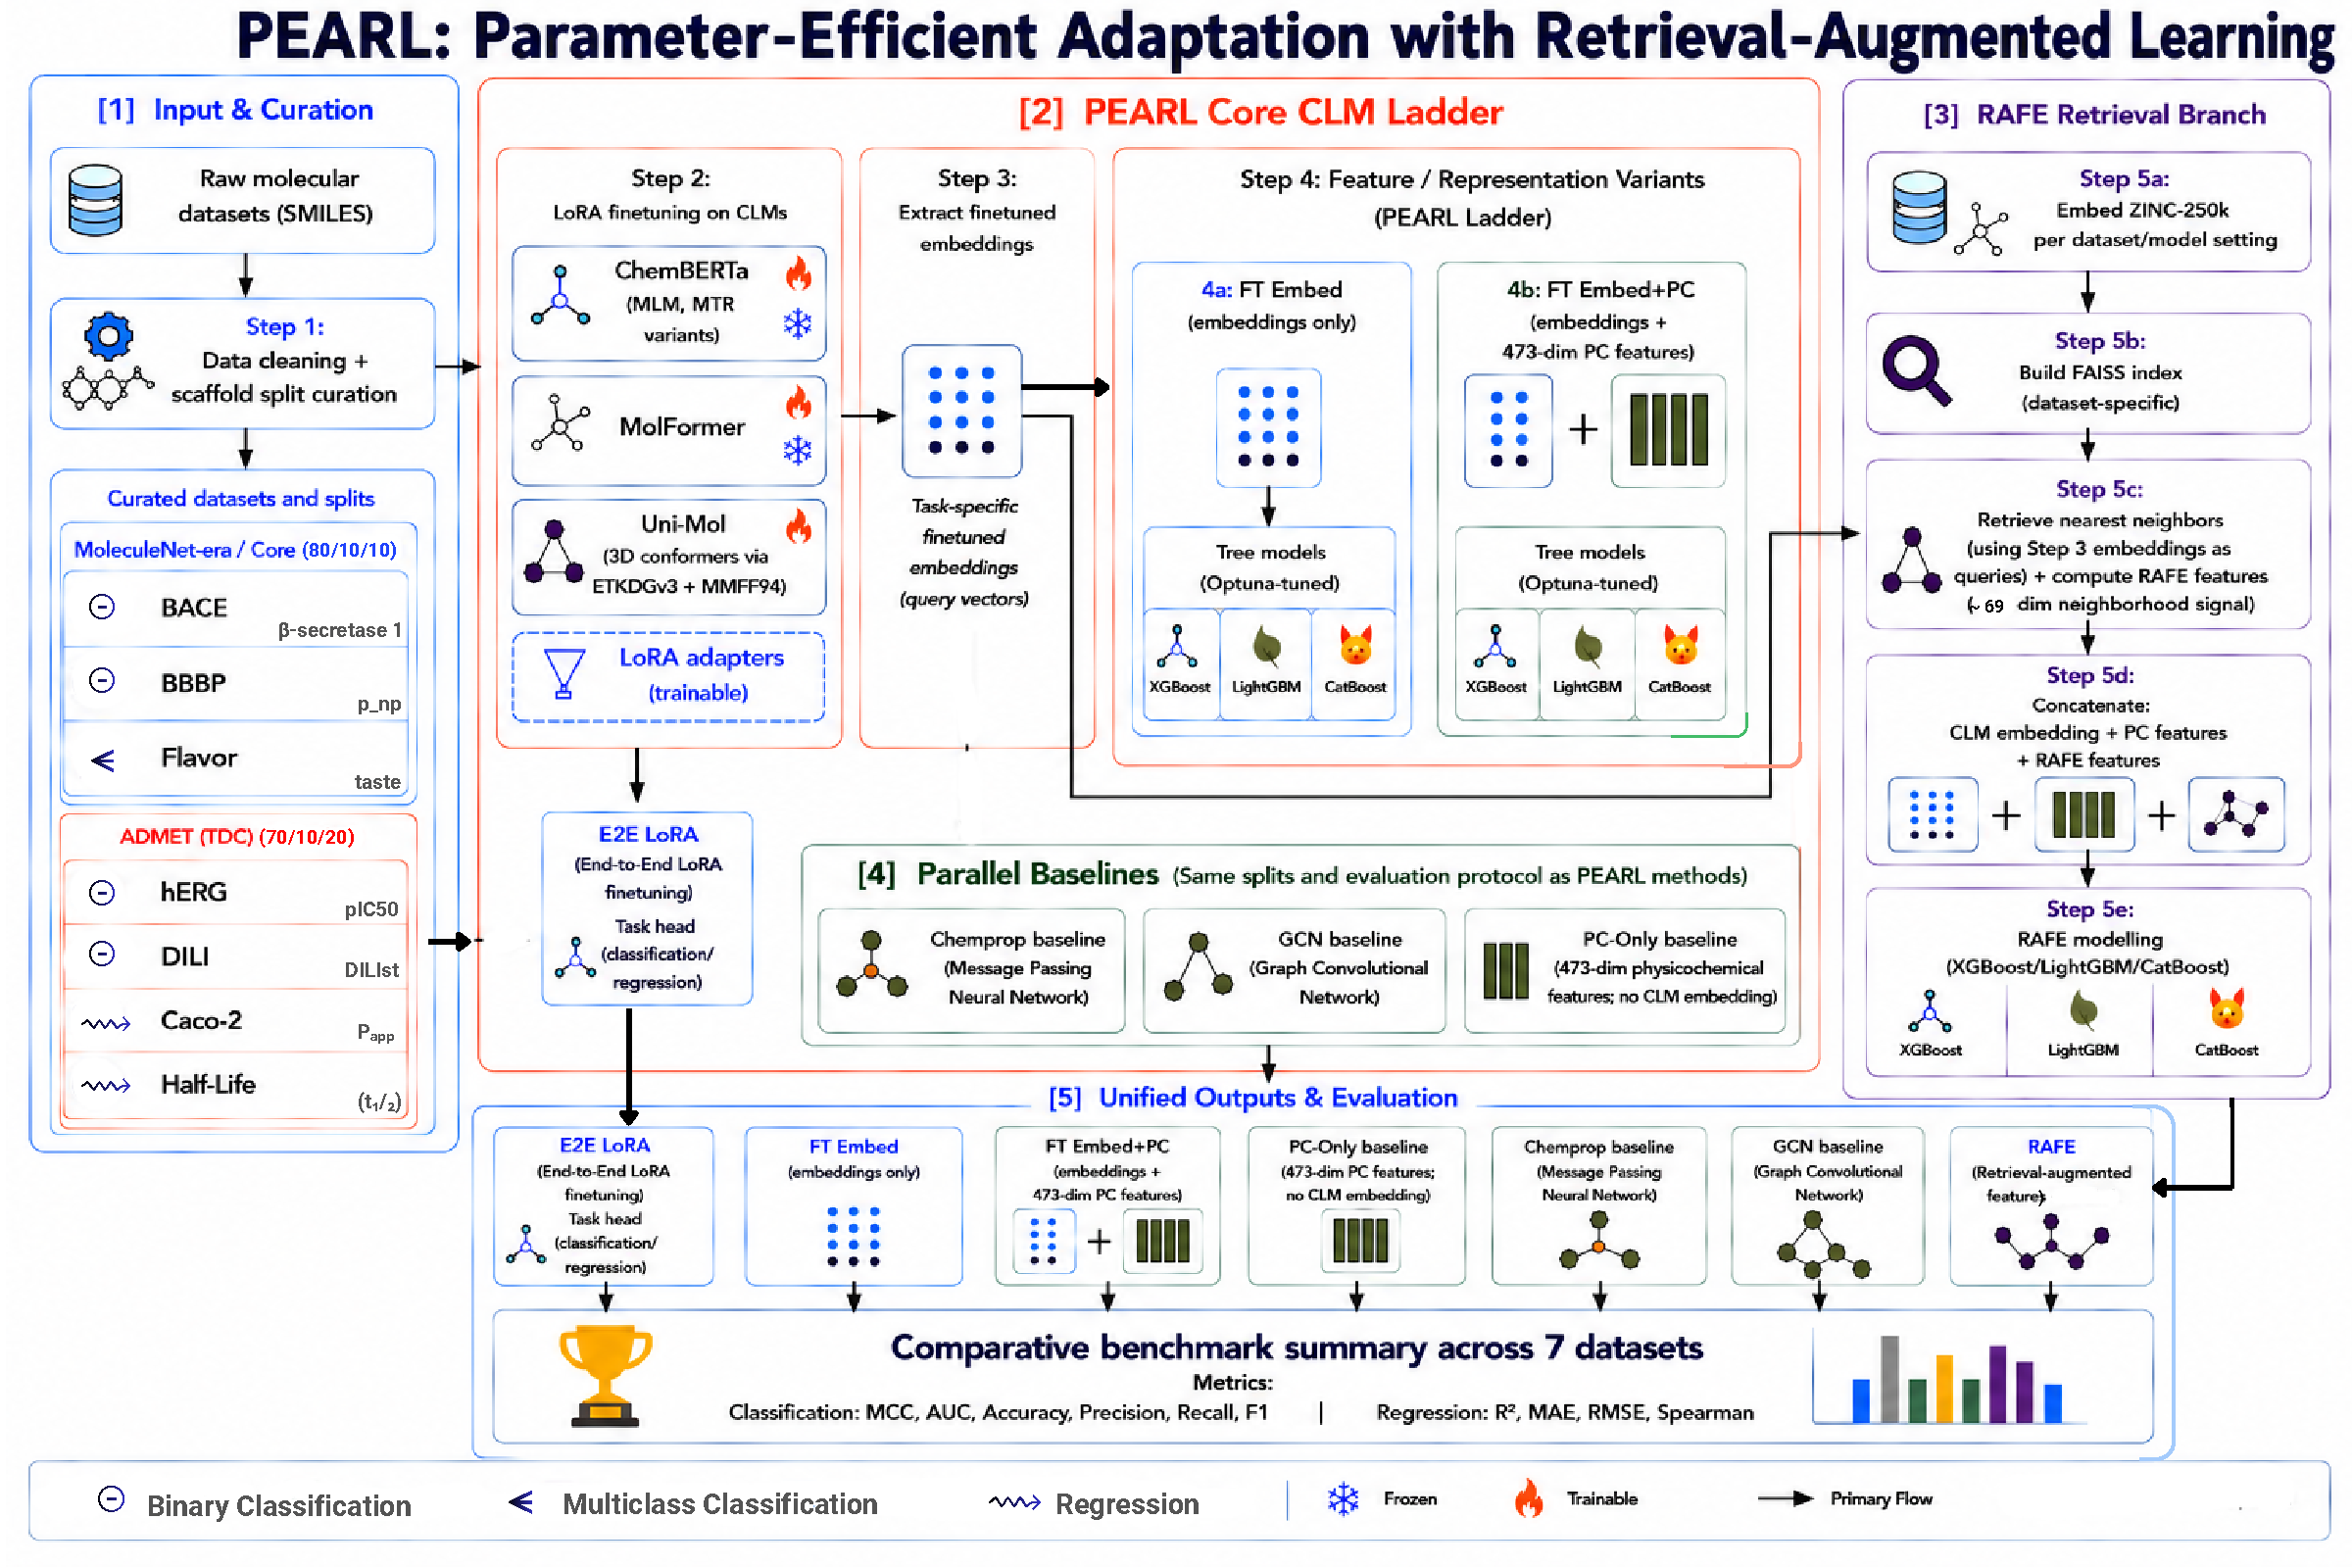
\includegraphics[width=0.98\textwidth]{Figures_v2/PEARL_Workflow_v2.pdf}
  \caption{PEARL workflow. Molecules are processed by one of three CLM families (ChemBERTa, MolFormer, Uni-Mol) with LoRA adapters. Task-specific embeddings are fused with molecular PC features and ZINC-250k retrieval features, then passed to tree-based classifiers/regressors. Uni-Mol additionally encodes 3D ETKDGv3 conformers via SE(3) representation. The ladder spans both classification and regression targets (including Caco-2, Half-Life) and is benchmarked against in-house Chemprop/GCN/PC-only baselines run under the same protocol.}
  \label{fig:workflow}
\end{figure*}

%% =====================================================================
\section{Related Work}\label{sec:related_work}

\subsection{Molecular Property Prediction}\label{sec:related_mpp}
ChemBERTa~\cite{chithrananda2020chemberta} and ChemBERTa-2~\cite{ahmad2022chemberta2} adapted BERT-style masked language modelling to SMILES, establishing the template for CLM pretraining on large molecular corpora. MolFormer~\cite{ross2022molformer} scaled this to $1.1\times10^9$ molecules using linear attention. Uni-Mol~\cite{zhou2023unimol} departed from SMILES by operating on explicit 3D atomic coordinates via an SE(3)-equivariant transformer, achieving state-of-the-art results on MoleculeNet through full finetuning. Multi-modal models such as MolT5~\cite{edwards2022molt5}, nach0~\cite{livne2024nach0}, and Omni-Mol~\cite{hu2025omnimol} further integrate SMILES, graphs, and natural language, but systematic evaluation under parameter-efficient conditions remains limited.

On the graph side, Chemprop~\cite{yang2019chemprop}, AttentiveFP~\cite{xiong2020attentivefp}, GROVER~\cite{rong2020grover}, and Mole-BERT~\cite{xia2023molecbert} all show how much graph-based molecular representations can offer. Rather than taking those numbers as reported in the original papers (Supplementary Section~S5), \textbf{PEARL additionally re-trains Chemprop and a GCN in-house}, on the exact same scaffold split, preprocessing, and bootstrapped-CI (confidence interval) protocol as every other method, on all seven datasets. The TDC~\cite{huang2021tdc} ADMET Group provides curated, leaderboard-tracked hERG~\cite{wang2016herg}, DILI~\cite{xu2019dili}, Caco-2~\cite{wang2016caco2}, and half-life~\cite{obach2008half} datasets, which broaden PEARL beyond MoleculeNet-era classification tasks and include regression targets.

\subsection{Parameter-Efficient Fine-Tuning (PEFT)}\label{sec:related_peft}
LoRA~\cite{hu2021lora} introduced low-rank weight updates for large language models; PEFT methods have since been evaluated for molecular tasks. Balne et al.~\cite{balne2024peft} and Xu et al.~\cite{xu2023peftreview} survey PEFT strategies broadly, including adapter layers, prefix tuning, and LoRA, while Fu et al.~\cite{fu2023effectiveness} assess their effectiveness in NLP. The work closest to ours is EffiChem~\cite{harod2025effichem}, which shows that LoRA-based adaptation of 1D CLMs (ChemBERTa, MolFormer) can be efficient for molecular property prediction.

PEARL goes considerably further along three axes. First, it adds Uni-Mol, a 3D SE(3)-equivariant model, enabling the first direct LoRA comparison between 1D SMILES-based and 3D geometry-aware CLMs on identical scaffold splits. Second, it introduces the RAFE framework, which augments frozen CLM embeddings with label-free chemical neighborhood features from an external knowledge base. Third, it benchmarks in-house GNN and PC-only baselines and extends the ladder to regression tasks. To our knowledge, no prior work combines PEFT with leakage-free retrieval augmentation across both 1D and 3D molecular representations and classification/regression tasks, under a fully in-house, identically-evaluated baseline suite.

\subsection{Retrieval-Augmented Generation (RAG) in Scientific ML}\label{sec:related_rag}
Generative RAG~\cite{lewis2020rag} conditions a language model on retrieved documents; molecular analogues typically retrieve labeled training-set molecules as auxiliary signals, introducing leakage and a small retrieval pool. KPGT~\cite{liu2022kpgt} injects knowledge-graph attributes into graph-transformer pretraining but retrieval occurs at pretraining time from the training corpus itself. PEARL's RAFE differs: it retrieves from a fixed external corpus (ZINC-250k) at inference time, extracts label-free physicochemical statistics as tree-model features, and applies to any CLM family without retraining.

%% =====================================================================
\section{The PEARL Framework}\label{sec:pearl_arch}

\subsection{Problem Formulation}\label{sec:problem_formulation}
Let $\mathcal{D} = \{(x_i, y_i)\}_{i=1}^{N}$ denote a molecular property dataset, where $x_i$ is the $i$-th molecule -- represented either as a SMILES string (ChemBERTa, MolFormer) or an explicit 3D atomic coordinate set obtained via conformer generation (Uni-Mol) -- and $y_i$ is its task-specific label. For binary classification tasks (BACE, BBBP, hERG, DILI), $y_i \in \{0,1\}$; for the multi-class Flavor task, $y_i \in \{1,\dots,5\}$; for regression tasks (Caco-2, Half-Life), $y_i \in \mathbb{R}$.

A pretrained CLM backbone $f_\theta : \mathcal{X} \rightarrow \mathbb{R}^{d}$ maps a molecule to a $d$-dimensional embedding ($d=384$ for ChemBERTa, $d=768$ for MolFormer, $d=2560$ for Uni-Mol's hybrid vector; Section~\ref{sec:pretrained_clms}). PEARL learns a task-specific predictor $g_\phi$ such that
\begin{equation}
  \hat{y}_i = g_\phi\big(h(x_i)\big), \qquad h(x_i) = f_\theta(x_i) \,\Vert\, p(x_i) \,\Vert\, r(x_i),
\end{equation}
where $\Vert$ denotes concatenation, $p(x_i) \in \mathbb{R}^{473}$ is an optional vector of engineered physicochemical descriptors (Section~\ref{sec:pearl_ladder}), and $r(x_i) \in \mathbb{R}^{69}$ is an optional RAFE feature vector obtained by retrieving the $k$ nearest neighbors of $x_i$ in an external corpus $\mathcal{Z}$ (ZINC-250k; Section~\ref{sec:rafe}). $\theta$ is adapted parameter-efficiently via low-rank updates $\Delta\theta$ with $|\Delta\theta| \ll |\theta|$ (Section~\ref{sec:lora}), and $\phi$ is optimized to minimize a task-appropriate loss $\mathcal{L}(\hat y_i, y_i)$ -- weighted cross-entropy or focal loss for classification, Huber loss for regression (Section~\ref{sec:loss_functions}). PEARL's four operational modes (Section~\ref{sec:pearl_ladder}) correspond to different choices of which terms in $h(x_i)$ are active and whether $g_\phi$ is trained end-to-end with $f_\theta$ or on frozen embeddings.

\subsection{Base CLM Backbone Architecture}\label{sec:pretrained_clms}
\textbf{ChemBERTa-2}~\cite{ahmad2022chemberta2} builds upon ChemBERTa~\cite{chithrananda2020chemberta} via a RoBERTa-style architecture trained on $77$ million canonical SMILES from PubChem~\cite{kim2023pubchem}. Two pretraining strategies are used: Masked Language Modeling (MLM) and Multi-Task Regression (MTR) on $200$ molecular property tasks. We use the two 77M-parameter variants, denoted \textbf{ChemBERTa-77M~MLM} and \textbf{ChemBERTa-77M~MTR}, each producing 384-dimensional embeddings.

\textbf{MolFormer}~\cite{ross2022molformer} is a scalable CLM that learns representations from SMILES without 3D geometry. It uses a transformer with linear attention (FAVOR+)~\cite{choromanski2021rethinking}, rotary positional embeddings~\cite{heo2024rotary}, and efficient distributed training~\cite{isard2009distributed}, enabling pretraining on $1.1\times 10^{9}$ molecules from PubChem~\cite{kim2023pubchem} and ZINC20~\cite{irwin2020zinc20}. We use the \textbf{MolFormer-XL-10pct-both} variant ($\approx 46$M parameters, pretrained on $10\%$ of both datasets) with 768-dimensional embeddings.

\textbf{Uni-Mol}~\cite{zhou2023unimol} is a universal 3D molecular pre-trained model based on a SE(3)-equivariant Transformer with 15 attention layers. Unlike SMILES-based CLMs, Uni-Mol accepts \emph{explicit 3D atomic coordinates} generated via RDKit ETKDGv3 conformer embedding followed by MMFF94 force-field minimization. This geometry-aware design gives Uni-Mol inductive biases suited to structure-dependent properties such as receptor binding affinity. For PEARL, each molecule is represented as a \textbf{2560-dimensional hybrid vector}: a 512-dimensional CLS token from the SE(3)-Transformer concatenated with 2048-dimensional Morgan ECFP4 fingerprints (radius $= 2$), combining 3D structural awareness with explicit 2D topological information.

\subsection{Parameter-Efficient Adaptation (LoRA)}\label{sec:lora}
Low-Rank Adaptation (LoRA)~\cite{hu2021lora} introduces two trainable low-rank matrices $\mathbf{A} \in \mathbb{R}^{d \times r}$ and $\mathbf{B} \in \mathbb{R}^{r \times d}$ alongside frozen pretrained weight matrices $\mathbf{W} \in \mathbb{R}^{d \times d}$ in the attention layers, where $r \ll d$ is the rank hyperparameter. The weight update is:
\begin{equation}
  \mathbf{W}' = \mathbf{W} + \Delta\mathbf{W}, \quad \Delta\mathbf{W} = \mathbf{A} \cdot \mathbf{B}.
\end{equation}
Matrix $\mathbf{A}$ is initialized from $\mathcal{N}(0, \sigma^2)$ and $\mathbf{B}$ from zeros, ensuring that adaptation begins from the pretrained representation.

\subsubsection{LoRA for ChemBERTa and MolFormer}
LoRA adapters are applied to the query ($\mathbf{W}^Q$), key ($\mathbf{W}^K$), and value ($\mathbf{W}^V$) projection matrices of each attention layer. All other parameters are frozen. Hyperparameter search covers rank $r \in \{4, 8, 16, 32, 64\}$, LoRA scaling $\alpha \in \{8, 16, 32, 64, 128\}$, and dropout $\in \{0.0, 0.1, 0.2\}$.

\subsubsection{LoRA for Uni-Mol}
The version of Uni-Mol employs a fused attention projection, where the query, key, and value transformations are combined into a single linear layer (\texttt{in\_proj}) rather than separate $\mathbf{W}^Q$, $\mathbf{W}^K$, and $\mathbf{W}^V$. Consequently, LoRA is applied directly to this unified projection module across all self-attention layers. Specifically, LoRA adapters are injected into the \texttt{in\_proj} weights (and \texttt{out\_proj} when available), enabling parameter-efficient fine-tuning without modifying the full backbone. The rank $r$ of the low-rank decomposition is selected from $\{4, 8, 16, 32\}$, while the scaling factor $\alpha$ is chosen from $\{8, 16, 32, 64\}$.

\begin{figure}[!htb]
  \centering
  \includegraphics[width=0.99\textwidth]{Figures_v2/LoRA_FineTuning_v2.pdf}
  \caption{Low-Rank Adaptation (LoRA) Architecture. A low-rank adaptation framework fine-tunes frozen transformer weights (Q/K/V layers) using trainable low-rank matrices (A, B), enabling efficient adaptation to task-specific molecular datasets, now including binary (hERG, DILI), multi-class (Flavor), and regression (Caco-2, Half-Life) targets.}
  \label{fig:lora-architecture}
\end{figure}
Conformers for all dataset molecules are generated once before the hyperparameter sweep and cached, avoiding redundant ETKDGv3 calls during hyperparameter optimization. We use necessary flags to prevent conformer generation failures for metal-coordinated SMILES. Figure~\ref{fig:lora-architecture} illustrates how LoRA finetuning is implemented within our framework. All models use AdamW with cosine-annealing learning rate schedules; the encoder (LoRA adapters) receives the base learning rate while the classification/regression head receives $5\times$ the base rate. Gradient clipping ($\text{max\_norm} = 1.0$) is applied over all parameters, and early stopping monitors validation MCC (classification) or validation RMSE (regression) with patience of 5 epochs. Bayesian hyperparameter optimization with WandB sweeps ($20$-$30$ trials per dataset) optimizes for the corresponding validation metric.

\subsection{Retrieval-Augmented Learning: the RAFE Component}\label{sec:rafe}

\subsubsection{Design Rationale and External Knowledge Base}\label{sec:zinc_rationale}
Naive retrieval-augmented approaches retrieve nearest neighbors from the task-specific training set and use their labels as auxiliary features. This introduces three problems: a small retrieval pool ($\sim$500-15,000 molecules depending on dataset), training-set leakage, and circular dependencies between the retrieval space and prediction target.

\noindent\textbf{Note on terminology:} Unlike generative RAG~\cite{lewis2020rag}, where retrieved passages are injected into a language model prompt, RAFE does not pass retrieved content to any neural model. Retrieved ZINC-250k neighbors serve solely as a source of label-free physicochemical statistics (logP, QED, SAS distributions, structural similarity) that are featurized and concatenated with the molecular embedding before a tree-based model. The ``retrieval-augmented'' framing refers to the use of an external knowledge base at inference time, not to in-context generation.

PEARL addresses all three problems by using \textbf{ZINC-250k}~\cite{gomez2018automatic} as the retrieval corpus, i.e.\ a curated subset of $249,455$ drug-like molecules from the ZINC database~\cite{irwin2020zinc20} with no overlap with any training, validation, or test split, across all seven PEARL datasets. Each ZINC-250k molecule carries three physicochemical properties: lipophilicity (logP), Quantitative Estimate of Drug-likeness (QED $\in [0,1]$), and Synthetic Accessibility Score (SAS $\in [1,10]$).

ZINC-250k is chosen as the retrieval corpus for four complementary reasons:
\begin{enumerate}
  \item \textbf{Scale and diversity:} $249,455$ drug-like molecules span a broad region of chemical space, providing a dense and representative neighborhood for any query molecule from any of the seven PEARL datasets (the largest, hERG, has 13,445 compounds; the smallest, DILI, has 475).
  \item \textbf{Zero leakage:} ZINC-250k has no label overlap with any training, validation, or test split used in this study. Retrieved neighbors cannot carry prediction targets, eliminating the circular dependency that plagues training-set retrieval.
  \item \textbf{Label-free property signal:} logP, QED, and SAS are computed directly from SMILES without biological assay data. Their distributions in the local neighborhood of a query molecule characterize its physico-chemical environment in a way that is complementary to the molecule's own PC features and to the CLM's learned representation.
  \item \textbf{Model-family independence:} ZINC-250k is embedded independently by each finetuned CLM variant (ChemBERTa, MolFormer, Uni-Mol) and for each dataset, yielding model- and dataset-specific FAISS indices. RAFE features are therefore always expressed in the same geometric space as the query molecule's embedding.
\end{enumerate}

\subsubsection{Vector Indexing with FAISS}\label{sec:vector_faiss}
For each of the seven datasets, ZINC-250k molecules are re-embedded using that dataset's task-specific finetuned model variants. For binary/multi-class tasks, this means six SMILES-based variants (ChemBERTa-MLM $\times$ 2 loss, ChemBERTa-MTR $\times$ 2 loss, MolFormer $\times$ 2 loss) plus two Uni-Mol variants (FL and WL). For the two regression datasets, only a single Huber-loss variant is finetuned per CLM family, yielding three SMILES-based and one Uni-Mol variant.

SMILES-based embeddings are 768-dimensional CLS tokens; Uni-Mol embeddings are 2560-dimensional hybrid vectors (512-dim SE(3)-Transformer CLS concatenated with 2048-dim ECFP4 fingerprints). Embeddings are L2-normalized and indexed with FAISS \texttt{GpuIndexFlatIP}~\cite{johnson2021faiss}, a GPU-accelerated exact cosine-similarity search that achieves sub-2~ms query latency at 249k$\times$768 on a single GPU. Indices are serialized as CPU \texttt{IndexFlatIP} files for portable, fast retrieval.

\subsubsection{Chemical Neighborhood Feature Extraction}\label{sec:feature_extraction}
For every molecule in every split (train, validation, test), each FAISS index is queried by cosine similarity for the $k \in \{10, 20\}$ nearest ZINC-250k neighbors ($k$ fixed by design across all seven datasets; see the discussion of this design choice as a study limitation in Section~\ref{sec:limitations}). Four feature groups are extracted:
\begin{itemize}
  \item[\textbf{(a)}] physico-chemical neighborhood profile ($\sim$27 features: mean/std of logP, QED, SAS at $k=10,20$, plus similarity-weighted means);
  \item[\textbf{(b)}] neighborhood density (5 features: nearest-neighbor similarity, mean/std of $k$-neighbor similarity at $k=10,20$);
  \item[\textbf{(c)}] embedding centroid features ($\sim$34 features: PCA-32 compression of the $k=10$ neighbor centroid, fit on train only, plus similarity-to-centroid and centroid spread via standard deviation);
  \item[\textbf{(d)}] Tanimoto structural similarity (3 features: Morgan-fingerprint Tanimoto to the top-1 and top-5 neighbors, plus Murcko-scaffold overlap fraction in the top-10).
\end{itemize}
Together these four groups yield a 69-dimensional RAFE feature vector per molecule, concatenated as: [$\text{CLM embeddings} \mid \text{PC features (473-dim)} \mid \text{ZINC RAFE features}$].

\begin{figure}[!ht]
  \centering
  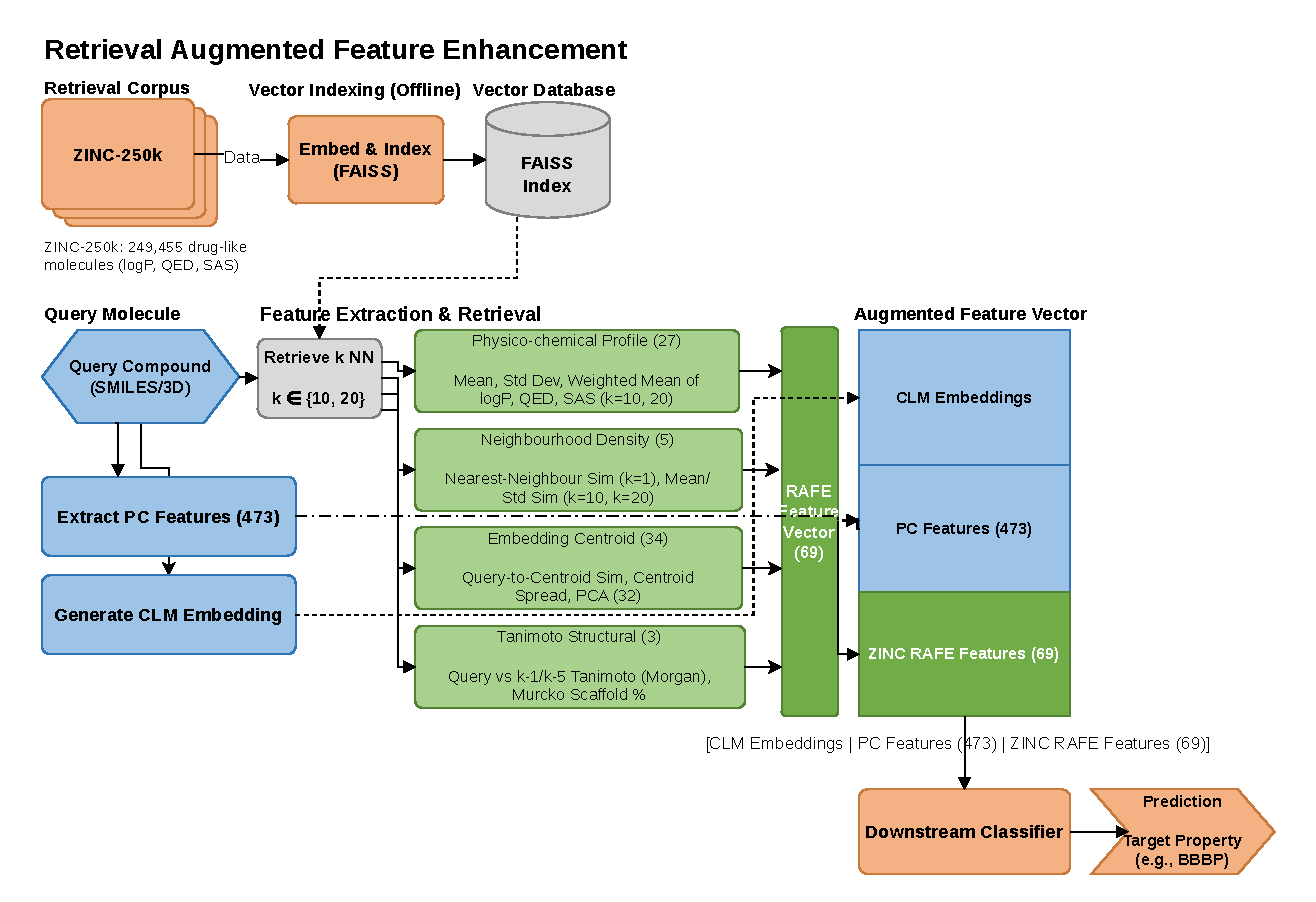
\includegraphics[width=0.99\textwidth]{Figures_v2/RAFE_Framework_v2.pdf}
  \caption{Retrieval-Augmented Feature Enhancement (RAFE) pipeline. A query molecule is embedded by a task-specific finetuned CLM; the embedding retrieves $k$ nearest chemical neighbors from the ZINC-250k FAISS index (re-built independently per dataset). Four feature groups are extracted (physico-chemical neighborhood profile, density/isolation, embedding centroid, Tanimoto similarity), yielding a 69-dim RAFE vector concatenated with the CLM embedding and PC features for tree-based classification or regression.}
  \label{fig:rafe}
\end{figure}

\subsection{PEARL Operational Ladder and Baselines}\label{sec:pearl_ladder}
PEARL defines four operational modes that form a progressive evaluation ladder, applicable to both classification and regression targets:

\textbf{(a)~End-to-End (E2E) LoRA finetuning:} The CLM backbone (ChemBERTa, MolFormer, or Uni-Mol) with LoRA adapters and a task-specific head is optimized end-to-end for each downstream task. For binary tasks, the head is a dense layer with sigmoid activation; for multi-class tasks, a dense layer with softmax; for regression tasks (Caco-2, Half-Life), a single linear output unit trained with Huber loss.

\textbf{(b)~Finetuned Embedding Prediction (FT~Embed):} Task-specific embeddings are extracted from the finetuned model. For MolFormer, the CLS token passes through two dense layers with GELU activation (768-dim output). For ChemBERTa, the CLS token passes through a dense layer with tanh activation (384-dim). For Uni-Mol, the CLS token is concatenated with ECFP4 fingerprints (2560-dim). These embeddings train Optuna-tuned~\cite{akiba2019optuna} tree-based classifiers (XGBoost / LightGBM / CatBoost) or, for the two regression datasets, their regressor counterparts.

\textbf{(c)~FT~Embed $+$ PC (Physicochemical Feature Fusion):} The FT~Embed vector is concatenated with 473~domain-specific physicochemical (PC) features: 148 RDKit molecular descriptors, 30 graph-based features (NetworkX v3.5.2), 128-bit Morgan fingerprints, and 167-bit MACCS keys (RDKit v2025.09.4). This combined vector trains the same tree-based models without any retrieval from external databases. A full description of engineered features is provided in Supplementary Table~S1.

\textbf{(d)~Retrieval-Augmented Feature Enhancement (RAFE):} RAFE augments the FT~Embed $+$ PC feature vector with ZINC-250k chemical neighborhood features (69-dim; Section~\ref{sec:rafe}), yielding the full feature vector [$\text{CLM embeddings} \mid \text{PC features (473-dim)} \mid \text{ZINC-250k RAFE features}$], passed to the same Optuna-tuned tree-based models.

\textbf{Baselines run in-house under the identical protocol, outside the ladder:} \textbf{PC-only} trains the same tree-model family directly on the 473-dim PC vector, with \emph{no} CLM component, isolating how much of the ladder's performance is attributable to the CLM. \textbf{Chemprop}~\cite{yang2019chemprop} (D-MPNN) and a \textbf{GCN} (GINConv-based, hand-rolled, atom/bond-featurized) are both trained end-to-end on the molecular graph, on the same scaffold split, with the same Optuna-style hyperparameter search budget and the same bootstrapped-CI evaluation as every CLM-based method above.

\subsection{Loss Functions for Class Imbalance and Regression}\label{sec:loss_functions}
Three loss functions address class imbalance (classification) or robust regression, implemented via a custom extension of the HuggingFace \texttt{Trainer}.

\noindent \textbf{Weighted cross-entropy (WL):} $\mathcal{L}_{\text{WL}} = -\sum_{i=0}^{C-1} w_i y_i \log\hat{y}_i$, where $w_i = 1 - f_i$ (inverse class frequency). This gives the minority class higher loss contribution and is most effective for datasets like BACE and Flavor.

\noindent\textbf{Focal loss (FL):} $\mathcal{L}_{\text{FL}} = -\alpha (1 - \hat{p}_i)^\gamma \log\hat{p}_i$ with $\gamma = 2$, which down-weights well-classified examples to focus learning on hard-to-classify boundary cases. This excels on heavily imbalanced and challenging classification tasks. hERG and DILI both use FL and WL sweeps, matching the same protocol used for BACE, BBBP, and Flavor.

\noindent\textbf{Huber loss (regression):} $\mathcal{L}_{\text{Huber}}(y, \hat y) = \begin{cases}\tfrac{1}{2}(y-\hat y)^2 & |y - \hat y| \le \delta \\ \delta(|y-\hat y| - \tfrac12 \delta) & \text{otherwise}\end{cases}$, with $\delta = 1.0$. Huber loss is used for both Caco-2 and Half-Life regression targets, combining MSE's smoothness near zero error with MAE's robustness to the outlier-prone tail of half-life measurements (Half-Life's target is additionally log1p-transformed before Huber loss is applied, and predictions are inverse-transformed before evaluation).

\subsection{Tree-Based Prediction Models}\label{sec:tree_models}
The final prediction stage employs XGBoost~\cite{chen2016xgboost}, LightGBM~\cite{ke2017lightgbm}, and CatBoost~\cite{prokhorenkova2018catboost}, in their classifier or regressor form as appropriate. These algorithms handle high-dimensional mixed-type feature vectors, provide built-in feature importance, and are robust to outliers. Bayesian hyperparameter optimization was performed with Optuna~\cite{akiba2019optuna} ($20$ trials for each configuration) maximizing validation MCC (classification, via stratified 5-fold CV) or minimizing validation RMSE (regression, via 5-fold CV). Class-weighting strategies address imbalance for classification tasks (\texttt{scale\_pos\_weight}, \texttt{class\_weight="balanced"}, \texttt{auto\_class\_weights="Balanced"} for XGBoost/LightGBM/CatBoost respectively); regression targets are otherwise unweighted.

%% =====================================================================
\section{Experimental Setup and Benchmarking}\label{sec:experimental_setup}

\subsection{Datasets}\label{sec:datasets}
The \textbf{Blood-Brain Barrier Penetration (BBBP)} dataset was originally curated in~\cite{martins2012bayesian} for predicting barrier permeability and contains over $2,000$ compounds with binary labels, integrated into the MoleculeNet~\cite{wu2018moleculenet} benchmark. The \textbf{Flavor Analysis and Recognition Transformer (FART)} dataset, introduced in~\cite{zimmermann2024fart}, is a multi-class taste prediction corpus of 15,025 compounds annotated as \textit{bitter}, \textit{sour}, \textit{sweet}, \textit{umami}, and \textit{undefined}. The \textbf{BACE} dataset is part of MoleculeNet~\cite{wu2018moleculenet} and contains experimentally measured binding results for 1,513 inhibitors of human $\beta$-secretase~1 (BACE-1), with binary activity labels. The dataset splits were curated using the DeepChem reference implementation~\cite{ramsundar2019deep}. BBBP is sourced from the IBM MolFormer repository and underwent validity checks, duplicate removal, and class-ambiguity filtering.

\textbf{TDC ADMET Group datasets:} Four datasets come from the Therapeutics Data Commons (TDC) ADMET Group~\cite{huang2021tdc}, chosen to broaden PEARL's task coverage beyond MoleculeNet-era binary/multi-class classification. These include \textbf{hERG}~\cite{wang2016herg} (binary, cardiac ion-channel inhibition, 13{,}445 compounds), \textbf{DILI}~\cite{xu2019dili} (binary, drug-induced liver injury, 475 compounds), \textbf{Caco-2}~\cite{wang2016caco2} (regression, log apparent permeability, 906 compounds), and \textbf{Half-Life}~\cite{obach2008half} (regression, plasma half-life in hours, 667 compounds). All four are curated via TDC's standard scaffold split and undergo the same SMILES standardization, validity filtering, and duplicate-removal pipeline used for BACE, BBBP, and Flavor. Half-Life additionally required IQR-based outlier removal in log1p space (bounds fit on the training split only, applied to all splits) to control the influence of a small number of extreme half-life values (max $\approx 1200$h vs.\ a $\sim$19h mean pre-filtering).

BBBP and BACE employ scaffold-based splits~\cite{ramsundar2019deep} using an 80:10:10 train/validation/test ratio. BBBP exhibits moderate class imbalance (78.8\% permeable in training); BACE is the most balanced, with $54.3\%$ inactive and $45.7\%$ active compounds, and its test set has $n\approx152$ molecules. The Flavor dataset uses the curated splits provided in~\cite{zimmermann2024fart}, with pronounced multi-class skew (sweet $41\%$, bitter $32\%$, sour $11\%$, umami $4\%$, undefined $12\%$) and $n_\text{test}=2{,}254$. The four TDC ADMET datasets use TDC's scaffold split (70:10:20 train/valid/test, the TDC ADMET Group default): hERG's test set ($n=2{,}690$) is class-imbalanced toward inhibitors ($\sim$70\%); DILI is the smallest classification dataset here ($n_\text{test}=96$), so its bootstrapped CIs are correspondingly the widest among the binary tasks; Caco-2 ($n_\text{test}=182$) and Half-Life ($n_\text{test}=133$) are both small regression sets, motivating the same bootstrapped-CI discipline applied throughout this study.

\begin{table}[!ht]
\centering
\caption{Structural summary of the seven PEARL benchmark datasets.}
\label{tab:dataset_summary}
\begin{adjustbox}{max width=\textwidth}
\begin{tabular}{lllll}
\toprule
Dataset & Task type & \# Compounds & Split (train:val:test) & Primary metric \\
\midrule
BACE       & Binary classification       & 1{,}513  & 80:10:10 ($n_\text{test}\approx152$)   & MCC \\
BBBP       & Binary classification       & $>$2{,}000 & 80:10:10                               & MCC \\
Flavor     & 5-class classification      & 15{,}025 & curated~\cite{zimmermann2024fart} ($n_\text{test}=2{,}254$) & MCC \\
hERG       & Binary classification       & 13{,}445 & 70:10:20 ($n_\text{test}=2{,}690$)      & MCC \\
DILI       & Binary classification       & 475      & 70:10:20 ($n_\text{test}=96$)           & MCC \\
Caco-2     & Regression (log permeability) & 906    & 70:10:20 ($n_\text{test}=182$)          & Spearman \\
Half-Life  & Regression (log1p, hours)   & 667      & 70:10:20 ($n_\text{test}=133$)          & Spearman \\
\bottomrule
\end{tabular}
\end{adjustbox}
\end{table}

\subsection{Baseline Models}\label{sec:baselines}
PEARL's four operational modes (Section~\ref{sec:pearl_ladder}) are compared against three in-house baselines run under the identical scaffold split, preprocessing, and evaluation protocol: \textbf{PC-only} (no CLM, no LoRA, no retrieval), \textbf{Chemprop}~\cite{yang2019chemprop} (D-MPNN), and a hand-rolled \textbf{GCN} (GINConv-based). Additionally, on the three MoleculeNet-era datasets (BACE, BBBP, Flavor) where comparable external LoRA/GNN literature numbers exist, PEARL is compared against published external baselines: Chemprop~\cite{yang2019chemprop}, GROVER~\cite{rong2020grover}, AttentiveFP~\cite{xiong2020attentivefp}, Mole-BERT~\cite{xia2023molecbert}, and the original Uni-Mol and MolFormer full-finetuning results (Section~\ref{sec:external_comparison}). The four TDC ADMET Group tasks have no comparable external LoRA/RAFE literature baseline, so their comparison is entirely in-house.

\subsection{Evaluation Protocol and Implementation Details}\label{sec:eval_protocol}
For classification, performance is evaluated using accuracy (Acc), area under the ROC curve (AUC), Matthews correlation coefficient (MCC), precision (Prec), recall (Rec), and F1-macro (F1$_\text{mac}$) / F1-micro (F1$_\text{mic}$); MCC is the primary ranking metric due to its robustness to class imbalance. For the two regression datasets (Caco-2, Half-Life), we report R\textsuperscript{2}, mean absolute error (MAE), and Spearman rank correlation.

Most datasets in this study have small-to-moderate test sets (DILI $n=96$; BACE $n\approx152$; Caco-2 $n=182$; Half-Life $n=133$), so \textbf{performance differences are interpreted alongside bootstrapped confidence intervals} (10{,}000 resamples, stratified by class label for classification, unstratified for regression with normal-approximation, computed on the fixed test-set predictions without retraining). We use a \textbf{$\pm 1$ SE} band for statistical difference during head-to-head comparisons.

All training uses AdamW with cosine-annealing learning rate schedules and Bayesian hyperparameter optimization via WandB sweeps ($20$-$30$ trials per dataset for LoRA finetuning) or Optuna~\cite{akiba2019optuna} ($20$ trials per configuration for the tree-based stage). Exact per-run hardware configuration, environment specification, and wall-clock timings are documented in the accompanying code repository (\url{https://github.com/raghvendra5688/PEARL}) to support full reproducibility.

%% =====================================================================
\section{Results and Discussion}\label{sec:results_discussion}

Results are organised around the four PEARL operational modes described in Section~\ref{sec:pearl_ladder}, plus the three in-house baselines (PC-only, Chemprop, GCN) run identically across all seven datasets: (i)~\textbf{E2E LoRA}: end-to-end LoRA finetuning of the CLM backbone; (ii)~\textbf{FT Embed}: Optuna-tuned tree models on frozen finetuned embeddings; (iii)~\textbf{FT Embed $+$ PC}: FT Embed augmented with 473-dim physicochemical features, without ZINC-250k retrieval; (iv)~\textbf{RAFE}: FT Embed $+$ PC further augmented with ZINC-250k neighborhood features. For each mode, we report the best-performing CLM variant and, where applicable, the corresponding tree model. Full ablation tables for each dataset are provided in the Supplementary Material.

\subsection{Main Benchmarking Results}\label{sec:main_results}

\subsubsection{Sequence of Comparisons}\label{sec:comparison_sequence}
The four PEARL modes form an evaluation ladder that isolates the contribution of each component, bracketed on one end by \textbf{PC-only} (no CLM at all) and on the other by \textbf{E2E LoRA} (fully differentiable gradient flow): \textbf{PC-only} establishes the floor achievable with no CLM -- any CLM-based method that fails to beat it has not demonstrated that its added architectural and computational complexity is earning its keep on that dataset. \textbf{E2E LoRA} establishes the ceiling achievable by fully differentiable gradient flow through the CLM backbone, treated as the upper bound for each CLM family and dataset. \textbf{FT Embed} quantifies how much embedding quality alone contributes; any gap between FT Embed and E2E LoRA reflects information recoverable only through end-to-end gradient flow. \textbf{FT Embed $+$ PC} isolates the contribution of physicochemical feature engineering, independent of any external retrieval. \textbf{RAFE} measures the additional value of ZINC-250k chemical neighborhood context: a gain from FT Embed $+$ PC to RAFE suggests that neighborhood signals from ZINC-250k provide information orthogonal to both the learned CLM representation and the molecule's own physicochemical profile. \textbf{Chemprop and GCN}, run in-house on the identical split and protocol, provide graph-based reference points that isolate the contribution of explicit bond-graph message passing, independent of any CLM pretraining corpus.

By applying a $\pm 1$~SE overlap test between each dataset's point-estimate winner and PC-only, \textbf{none of the four TDC ADMET datasets (hERG, DILI, Caco-2, Half-Life) shows a statistically confirmed win over PC-only}: every point-estimate winner's $\pm 1$~SE band overlaps PC-only's. This mirrors the pattern already observed for Flavor. Figure~\ref{fig:results_summary} summarizes the mean$\pm$SE primary metric for every method across all seven datasets.

\begin{figure*}[!ht]
  \centering
  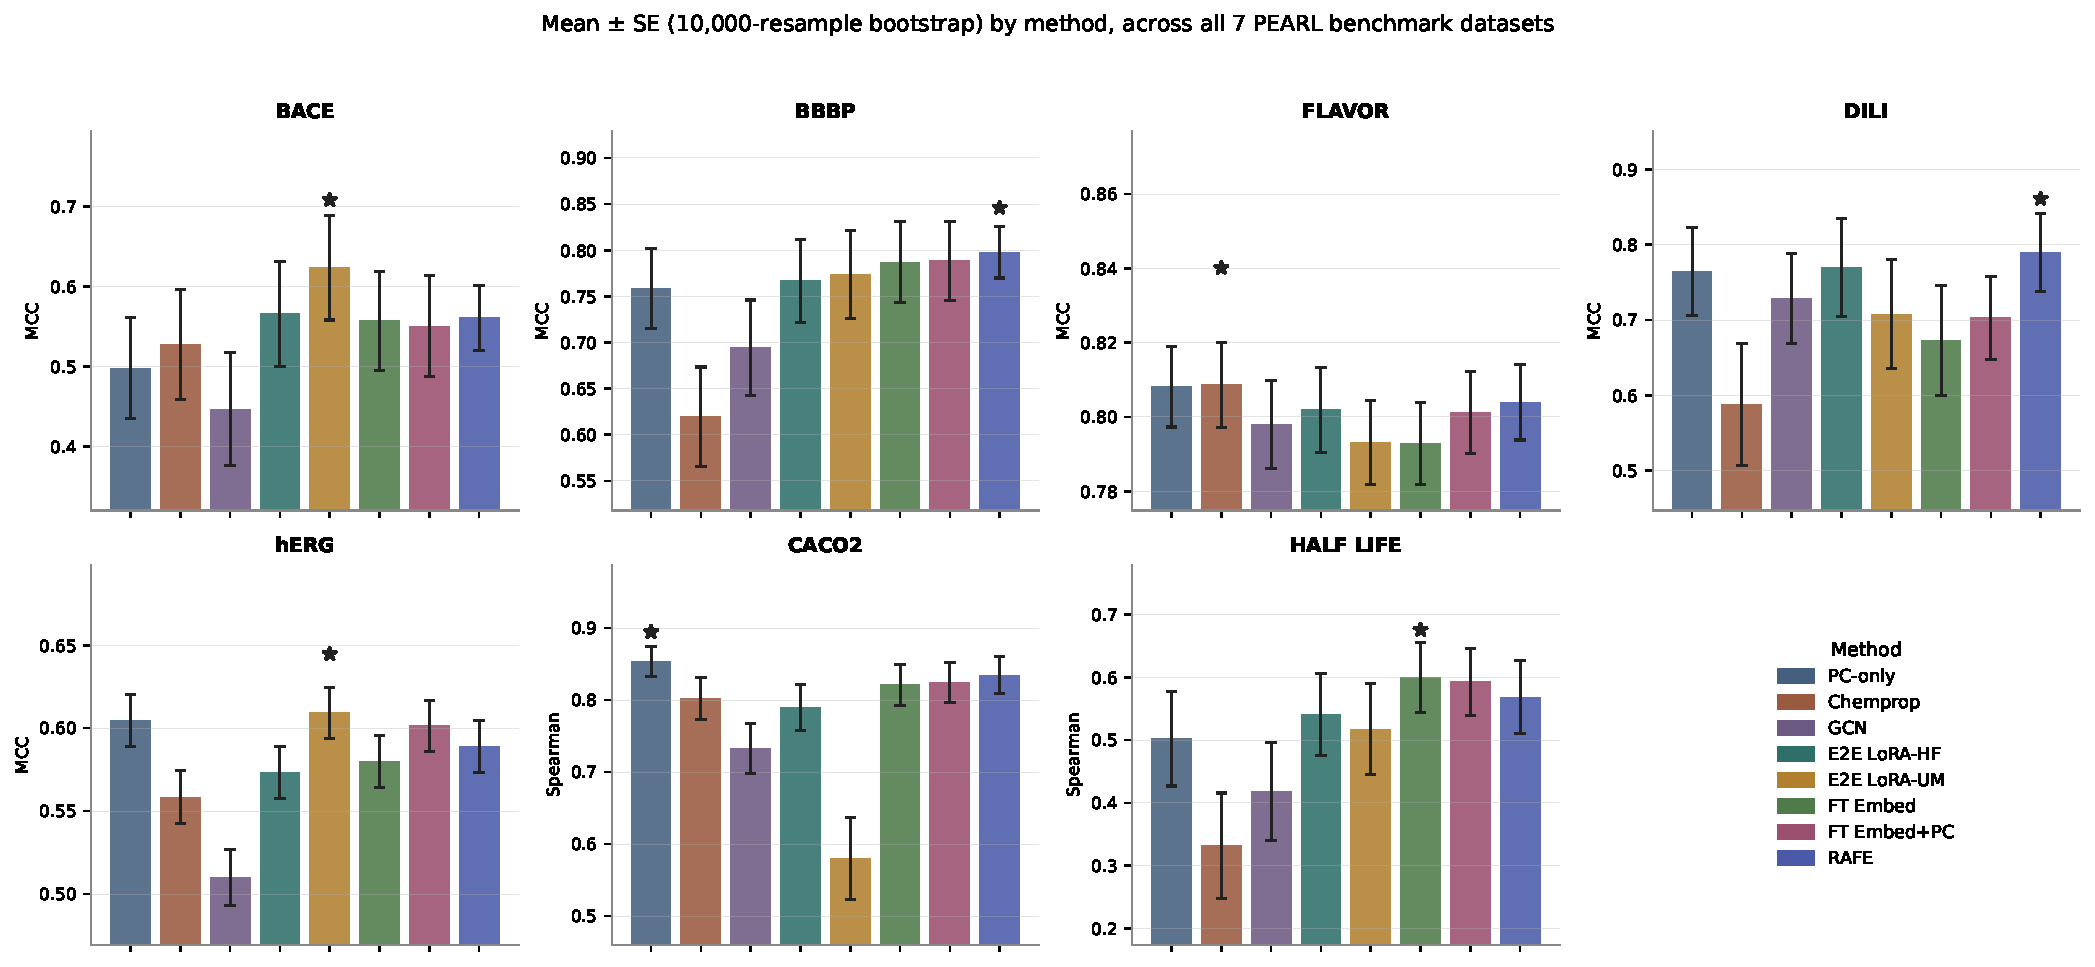
\includegraphics[width=0.99\textwidth]{Figures_v2/results_summary_v2.pdf}
  \caption{Mean $\pm$ SE (10,000-resample bootstrap) of the primary ranking metric (MCC for classification, Spearman for regression) for every method across all seven PEARL benchmark datasets. Stars mark the point-estimate winner per dataset. Whisker overlap between the winner and PC-only means the win is not statistically confirmed at $\pm1$~SE; this is the case for six of seven datasets (all but BACE).}
  \label{fig:results_summary}
\end{figure*}

\subsubsection{BBBP Dataset Results}
Table~\ref{tab:bbbp} presents the best configuration per modality and CLM family for BBBP. \textbf{RAFE with MolFormer-XL (FL~+~XGBoost) achieves the best overall result} (MCC$=0.798$, AUC$=0.940$, SE$=0.028$), $\approx 4\%$ ahead of E2E LoRA MolFormer FL (MCC$=0.767$, AUC$=0.929$) and Uni-Mol E2E LoRA WL (MCC$=0.774$, AUC$=0.943$) w.r.t. MCC metric. RAFE's gain over FT Embed+PC (MolFormer-XL FL + LightGBM, MCC$=0.789$) and over Uni-Mol RAFE (FL + XGBoost, MCC$=0.773$) points to ZINC-250k neighborhood context -- high mean logP of retrieved neighbors, associated with BBB-permeable molecules -- as an interpretable, complementary signal. PC-only is a strong baseline here too (MCC$=0.759$, AUC$=0.937$): RAFE's point-estimate gain over it is $+0.039$ MCC, and their $\pm1$~SE bands ($0.798\pm0.028$ vs.\ $0.759\pm0.043$) are close to non-overlapping, the strongest of the two confirmed-adjacent ``wins'' reported in this paper. Full per-embedding, per-loss ablation is in Supplementary Table~S2.

\begin{table*}[!ht]
\centering
\caption{Best performing configurations for each modality/baseline on BBBP. $^*$ denotes overall best by MCC. RAFE = FT~Embed~+~PC~+~ZINC-250k retrieval features. PC-only / Chemprop / GCN are run in-house on the identical split.}
\label{tab:bbbp}
\begin{adjustbox}{max width=\textwidth}
\begin{tabular}{lllllrrrrrrr}
\toprule
Modality & CLM & Loss & ML & AUC & Acc & F1$_\text{mac}$ & F1$_\text{mic}$ & MCC & Prec & Rec & SE(MCC) \\
\midrule
PC-only    & --- & --- & LightGBM & 0.937 & 0.885 & 0.867 & 0.885 & 0.759 & 0.916 & 0.846 & 0.043 \\
Chemprop   & --- & --- & --- & 0.918 & 0.807 & 0.801 & 0.807 & 0.620 & 0.799 & 0.821 & 0.054 \\
GCN        & --- & --- & --- & 0.924 & 0.859 & 0.839 & 0.859 & 0.694 & 0.874 & 0.822 & 0.052 \\
\midrule
E2E LoRA   & MolFormer-XL & FL & --- & 0.929 & 0.891 & 0.874 & 0.891 & 0.767 & 0.913 & 0.856 & 0.045 \\
E2E LoRA   & Uni-Mol      & WL & --- & 0.943 & 0.896 & 0.887 & 0.896 & 0.774 & 0.890 & \textbf{0.885} & 0.048 \\
\midrule
FT Embed   & MolFormer-XL & FL & XGBoost & 0.935 & 0.901 & 0.888 & 0.901 & 0.787 & 0.914 & 0.873 & 0.044 \\
FT Embed+PC& MolFormer-XL & FL & LightGBM& 0.934 & 0.901 & 0.887 & 0.901 & 0.789 & 0.920 & 0.870 & 0.043 \\
\midrule
RAFE$^*$   & MolFormer-XL & FL & XGBoost & \textbf{0.940} & \textbf{0.906} & \textbf{0.895} & \textbf{0.906} & \textbf{0.798} & \textbf{0.918} & 0.881 & \textbf{0.028} \\
RAFE       & Uni-Mol      & FL & XGBoost & 0.928 & 0.891 & 0.872 & 0.891 & 0.773 & 0.927 & 0.850 & --- \\
\bottomrule
\end{tabular}
\end{adjustbox}
\end{table*}

\subsubsection{Flavor Dataset Results}
Table~\ref{tab:flavor} presents results on the multi-class Flavor dataset. \textbf{RAFE (MolFormer-XL WL + CatBoost) achieves MCC$=0.804$} (AUC$=0.963$, Prec$=0.868$, Rec$=0.749$, SE$=0.010$), statistically indistinguishable from Chemprop (MCC$=0.809$, SE$=0.0115$) and PC-only (MCC$=0.808$, SE$=0.0108$) at $\pm1$~SE -- all four bands overlap heavily on this large ($n_\text{test}=2{,}254$), well-powered test set. This is a dataset where the CLM ladder does not clear the PC-only / GNN baselines by any meaningful margin. Uni-Mol reaches MCC$=0.795$ with weighted loss, competitive with but below MolFormer, a sign that 3D geometry does not add much for taste prediction. Full per-embedding, per-loss ablation is in Supplementary Table~S3.

\begin{table*}[t]
\centering
\caption{Best performing configurations on Flavor. Prec/Rec are macro-averaged; AUC is one-vs-rest macro ROC AUC.}
\label{tab:flavor}
\begin{adjustbox}{max width=\textwidth}
\begin{tabular}{lllllrrrrrrr}
\toprule
Modality & CLM & Loss & ML & AUC & Acc & F1$_\text{mac}$ & F1$_\text{mic}$ & MCC & Prec & Rec & SE(MCC) \\
\midrule
PC-only    & --- & --- & XGBoost  & 0.972 & 0.890 & 0.761 & 0.890 & 0.808 & 0.733 & 0.798 & 0.0108 \\
Chemprop   & --- & --- & --- & 0.974 & \textbf{0.899} & \textbf{0.809} & \textbf{0.899} & \textbf{0.809} & 0.796 & 0.835 & 0.0115 \\
GCN        & --- & --- & --- & 0.973 & 0.893 & 0.814 & 0.893 & 0.798 & 0.834 & 0.800 & 0.0118 \\
\midrule
E2E LoRA   & MolFormer-XL & WL & --- & \textbf{0.975} & 0.892 & \textbf{0.809} & 0.892 & 0.802 & 0.802 & 0.817 & 0.0115 \\
\midrule
FT Embed   & MolFormer-XL & WL & LightGBM& 0.970 & 0.882 & 0.783 & 0.882 & 0.787 & 0.800 & 0.778 & 0.0111 \\
FT Embed+PC& MolFormer-XL & WL & CatBoost& 0.958 & 0.888 & 0.772 & 0.888 & 0.801 & 0.756 & 0.793 & 0.0111 \\
\midrule
RAFE       & MolFormer-XL & WL & CatBoost& 0.963 & 0.893 & 0.774 & 0.893 & 0.804 & \textbf{0.868} & 0.749 & 0.0102 \\
\bottomrule
\end{tabular}
\end{adjustbox}
\end{table*}

\subsubsection{BACE Dataset Results}
Table~\ref{tab:bace} compares key configurations on BACE. BACE remains the most challenging dataset here (MCC $< 0.65$ across all methods). Figure~\ref{fig:bace} compares the AUC and AUPR of Uni-Mol E2E LoRA with counterparts in the CLM ladder. \textbf{Uni-Mol with weighted loss achieves the best overall performance} (MCC$=0.623$, SE$=0.039$; AUC$=0.891$; Acc$=0.822$), an 8\% absolute MCC gain over the next-best SMILES-based E2E LoRA (MolFormer-XL FL, MCC$=0.566$, SE$=0.066$) and over PC-only (MCC$=0.498$, SE$=0.063$). The $\pm1$~SE bands of Uni-Mol and MolFormer FL overlap ($0.623\pm0.039$ vs.\ $0.566\pm0.066$), so the gain over the best SMILES-based method is directionally consistent but not statistically confirmed on this $n=152$ test set; the gain of Uni-Mol over PC-only, however, is large enough that their $\pm1$~SE bands do not overlap ($0.623\pm0.039$ vs.\ $0.498\pm0.063$), making BACE the clearest confirmed win for the CLM ladder over the no-CLM baselines. This is consistent with BACE-1 inhibitor activity being governed by 3D ligand-receptor complementarity.

RAFE with MolFormer-XL (WL~+~LightGBM) achieves MCC$=0.561$, SE$=0.040$, intermediate between FT Embed (MCC$=0.557$) and E2E LoRA (MCC$=0.566$), and does not close the gap to Uni-Mol E2E LoRA. Full per-embedding, per-loss ablation results are reported in Supplementary Table~S4.

\begin{figure*}[!ht]
  \centering
  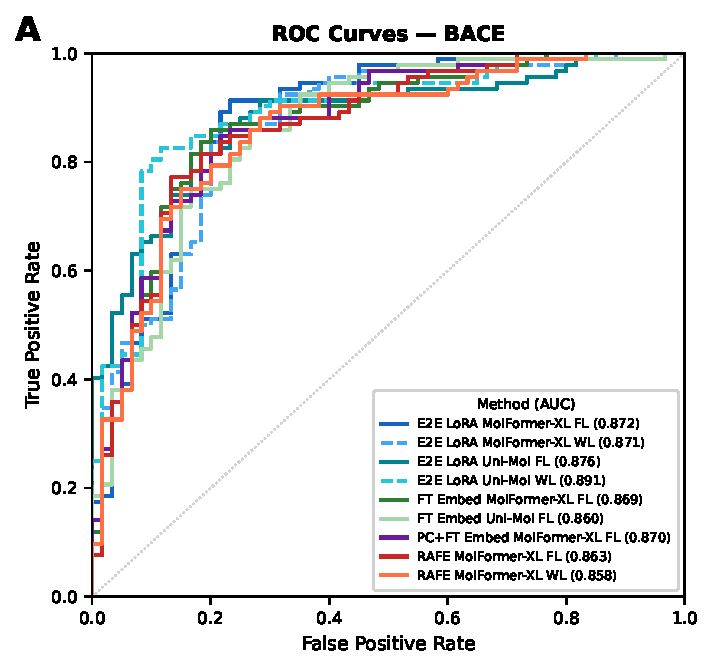
\includegraphics[width=0.49\textwidth]{Figures_v2/bace_roc.pdf}
  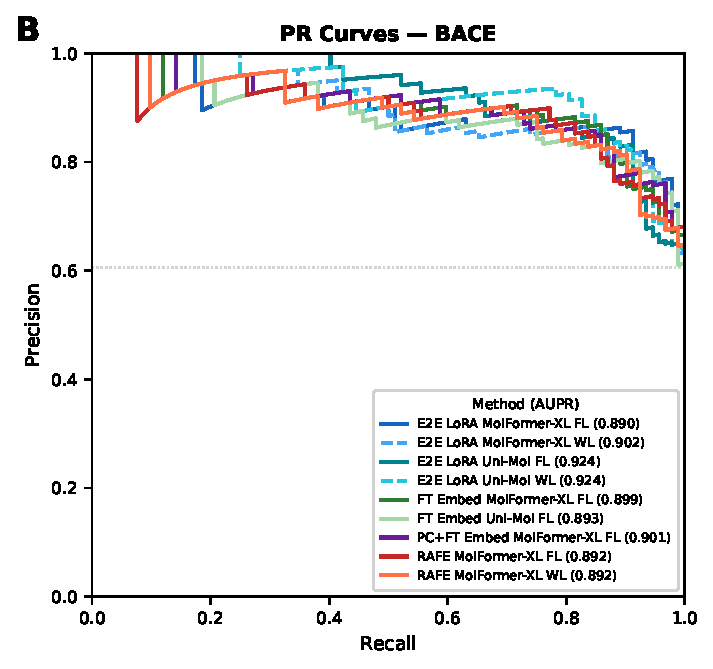
\includegraphics[width=0.49\textwidth]{Figures_v2/bace_pr.pdf}
  \caption{ROC and precision-recall curves for BACE inhibitor prediction. Uni-Mol WL achieves the highest AUPR and overall MCC~$=0.623$.}
  \label{fig:bace}
\end{figure*}

\begin{table*}[ht]
\centering
\caption{Best configurations on BACE. $^*$ overall best by MCC.}
\label{tab:bace}
\begin{adjustbox}{max width=\textwidth}
\begin{tabular}{lllllrrrrrrr}
\toprule
Modality & CLM & Loss & ML & AUC & Acc & F1$_\text{mac}$ & F1$_\text{mic}$ & MCC & Prec & Rec & SE(MCC) \\
\midrule
PC-only    & --- & --- & CatBoost & 0.850 & 0.724 & 0.723 & 0.724 & 0.498 & 0.746 & 0.751 & 0.063 \\
Chemprop   & --- & --- & --- & 0.855 & 0.763 & 0.759 & 0.763 & 0.528 & 0.758 & 0.770 & 0.068 \\
GCN        & --- & --- & --- & 0.795 & 0.717 & 0.714 & 0.717 & 0.447 & 0.719 & 0.729 & 0.071 \\
\midrule
E2E LoRA   & MolFormer-XL & FL & --- & 0.872 & 0.789 & 0.785 & 0.789 & 0.566 & 0.783 & 0.789 & 0.066 \\
E2E LoRA$^*$ & Uni-Mol    & WL & --- & \textbf{0.891} & \textbf{0.822} & \textbf{0.808} & \textbf{0.822} & \textbf{0.623} & \textbf{0.823} & \textbf{0.801} & \textbf{0.039} \\
\midrule
FT Embed   & MolFormer-XL & FL & CatBoost & 0.869 & 0.763 & 0.762 & 0.763 & 0.557 & 0.773 & 0.784 & 0.062 \\
RAFE       & MolFormer-XL & WL & LightGBM & 0.858 & 0.770 & 0.768 & 0.770 & 0.561 & 0.774 & 0.787 & 0.040 \\
\bottomrule
\end{tabular}
\end{adjustbox}
\end{table*}

\subsubsection{TDC ADMET Group Results}\label{sec:new_datasets}
This section reports results on the four TDC ADMET Group datasets. All four are evaluated with the same in-house PC-only, Chemprop, and GCN baselines as BACE/BBBP/Flavor.

\paragraph{hERG (Cardiac Ion-Channel Inhibition).} Table~\ref{tab:herg} shows results for the hERG dataset. \textbf{Uni-Mol E2E LoRA (WL) is the point-estimate winner} (MCC$=0.609$, AUC$=0.881$, SE$=0.0154$), narrowly ahead of PC-only (MCC$=0.604$, SE$=0.0157$), FT~Embed+PC (Uni-Mol FL + LightGBM, MCC$=0.602$, SE$=0.0154$), and RAFE (Uni-Mol FL + LightGBM, MCC$=0.589$, SE$=0.0155$). \textbf{All four bands overlap at $\pm 1$~SE}: on hERG's large, well-powered test set ($n=2{,}690$), the absolute MCC gaps are tiny (0.005-0.020) relative to the whisker widths, so this is not a statistically confirmed win for any CLM-based method over the PC-only classifier. Full set of ablations in Supplementary Table~S5.

\begin{table*}[!ht]
\centering
\caption{Best configurations on hERG (binary, cardiac ion-channel inhibition).}
\label{tab:herg}
\begin{adjustbox}{max width=\textwidth}
\begin{tabular}{lllllrrrrrrr}
\toprule
Modality & CLM & Loss & ML & AUC & Acc & F1$_\text{mac}$ & MCC & Prec & Rec & SE(MCC) \\
\midrule
PC-only     & --- & --- & XGBoost  & 0.874 & 0.802 & 0.802 & 0.604 & 0.802 & 0.802 & 0.0157 \\
Chemprop    & --- & --- & ---      & 0.854 & 0.779 & 0.779 & 0.558 & 0.779 & 0.779 & 0.0160 \\
GCN         & --- & --- & ---      & 0.833 & 0.755 & 0.755 & 0.510 & 0.755 & 0.755 & 0.0168 \\
\midrule
E2E LoRA    & MolFormer-XL & WL & --- & 0.869 & 0.787 & 0.787 & 0.573 & 0.787 & 0.787 & 0.0155 \\
E2E LoRA$^*$& Uni-Mol      & WL & --- & \textbf{0.881} & \textbf{0.804} & \textbf{0.804} & \textbf{0.609} & \textbf{0.805} & \textbf{0.804} & \textbf{0.0154} \\
\midrule
FT Embed    & Uni-Mol & FL & LightGBM & 0.864 & 0.790 & 0.790 & 0.580 & 0.790 & 0.790 & 0.0158 \\
FT Embed+PC & Uni-Mol & FL & LightGBM & 0.871 & 0.801 & 0.801 & 0.602 & 0.801 & 0.801 & 0.0154 \\
RAFE        & Uni-Mol & FL & LightGBM & 0.871 & 0.794 & 0.794 & 0.589 & 0.794 & 0.795 & 0.0155 \\
\bottomrule
\end{tabular}
\end{adjustbox}
\end{table*}

\paragraph{DILI (Drug-Induced Liver Injury).} Table~\ref{tab:dili} shows results for the DILI dataset. \textbf{RAFE (Uni-Mol FL + XGBoost) is the point-estimate winner} (MCC$=0.790$, AUC$=0.875$, SE$=0.0515$), ahead of E2E LoRA (ChemBERTa-MTR WL, MCC$=0.770$) and PC-only (MCC$=0.765$, SE$=0.0581$). This is the largest absolute point-estimate gap of any dataset in this group ($+0.025$ MCC over PC-only). But DILI's small test set ($n=96$) gives every method a wide SE ($\ge0.05$), and RAFE's $\pm1$~SE band ($0.790\pm0.052$) overlaps PC-only's ($0.765\pm0.058$), so even the largest margin among the four TDC ADMET datasets remains an unconfirmed win. Full set of ablation results are provided in Supplementary Table~S6.

\begin{table*}[!ht]
\centering
\caption{Best configurations on DILI (binary, drug-induced liver injury, TDC ADMET Group).}
\label{tab:dili}
\begin{adjustbox}{max width=\textwidth}
\begin{tabular}{lllllrrrrrrr}
\toprule
Modality & CLM & Loss & ML & AUC & Acc & F1$_\text{mac}$ & MCC & Prec & Rec & SE(MCC) \\
\midrule
PC-only     & --- & --- & CatBoost & 0.914 & 0.875 & 0.872 & 0.765 & 0.894 & 0.870 & 0.0581 \\
Chemprop    & --- & --- & ---      & 0.893 & 0.792 & 0.788 & 0.588 & 0.800 & 0.788 & 0.0808 \\
GCN         & --- & --- & ---      & 0.889 & 0.854 & 0.850 & 0.729 & 0.880 & 0.849 & 0.0600 \\
\midrule
E2E LoRA    & ChemBERTa-MTR & WL & --- & 0.911 & \textbf{0.885} & \textbf{0.885} & 0.770 & 0.886 & \textbf{0.885} & 0.0650 \\
E2E LoRA    & Uni-Mol       & FL & --- & \textbf{0.926} & 0.854 & 0.854 & 0.708 & 0.855 & 0.853 & 0.0722 \\
\midrule
FT Embed    & ChemBERTa-MLM & WL & CatBoost & 0.893 & 0.833 & 0.831 & 0.673 & 0.844 & 0.830 & 0.0731 \\
FT Embed+PC & Uni-Mol       & FL & LightGBM & 0.873 & 0.833 & 0.826 & 0.703 & 0.879 & 0.826 & 0.0552 \\
RAFE$^*$    & Uni-Mol       & FL & XGBoost  & 0.875 & \textbf{0.885} & 0.883 & \textbf{0.790} & \textbf{0.910} & 0.880 & \textbf{0.0515} \\
\bottomrule
\end{tabular}
\end{adjustbox}
\end{table*}

Figures~\ref{fig:roc_4ds} and~\ref{fig:pr_4ds} summarize the four tree-based modalities (PC-only, FT Embed, FT Embed+PC, RAFE) across all four binary classification datasets, and two things stand out. First, on hERG the four ROC and PR curves are nearly superimposed (AUC $0.864$-$0.874$, AUPR $0.862$-$0.872$), consistent with the $\pm1$~SE overlap already reported: none of the tree-based modalities separates meaningfully from PC-only on this large, well-powered test set. Second, RAFE's ranking among the tree-based modalities is dataset-dependent rather than uniformly best. It is the top tree-based modality on BBBP (AUC$=0.940$, AUPR$=0.940$), but on BACE it is the weakest of the four (AUC$=0.858$, trailing FT Embed and FT Embed+PC at $0.869$-$0.870$). That is fitting, since BACE's confirmed win traces back to the 3D Uni-Mol E2E LoRA model, not to tree-based RAFE. DILI shows the largest divergence between the two curve types: PC-only's AUC margin over RAFE is modest ($0.914$ vs.\ $0.875$), but its AUPR margin is substantially larger ($0.911$ vs.\ $0.847$). This shows that on this small ($n=96$), imbalanced test set PC-only's precision-recall trade-off is more favorable than ROC-AUC alone would suggest, even though RAFE remains the point-estimate MCC winner in Table~\ref{tab:dili}.

\begin{figure*}[!ht]
  \centering
  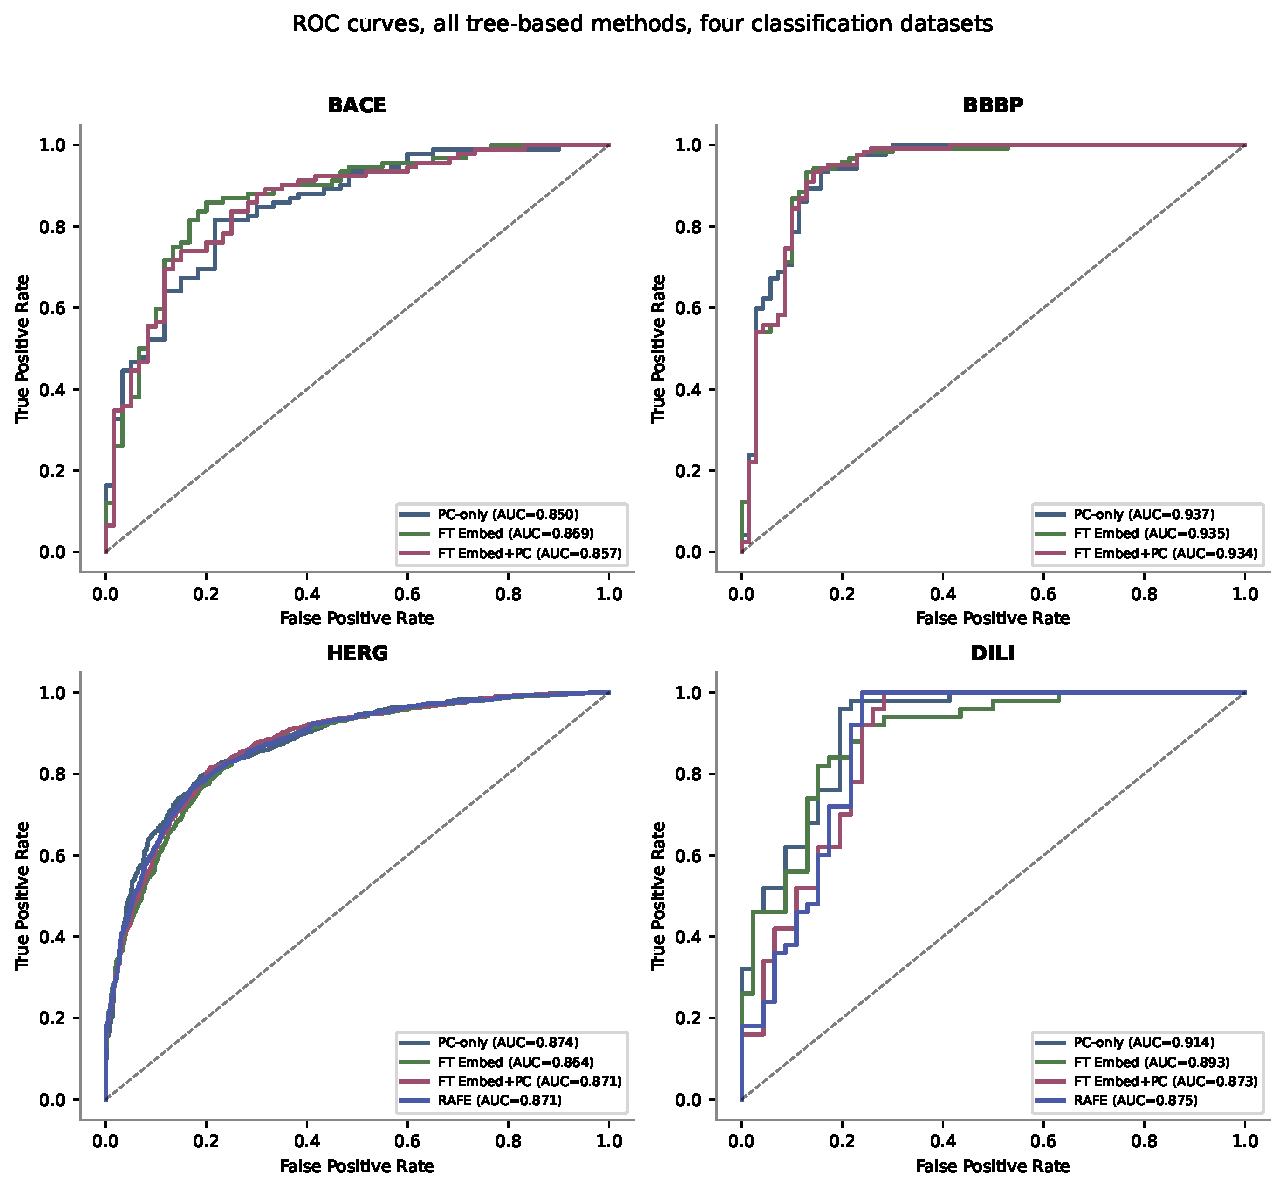
\includegraphics[width=0.95\textwidth]{Figures_v2/roc_curves_4datasets.pdf}
  \caption{ROC curves for best configuration of tree-based methods (PC-only, FT Embed, FT Embed+PC and RAFE), on all four binary classification datasets in this study: two MoleculeNet (BACE, BBBP) and two TDC ADMET tasks (hERG, DILI).}
  \label{fig:roc_4ds}
\end{figure*}

\begin{figure*}[!ht]
  \centering
  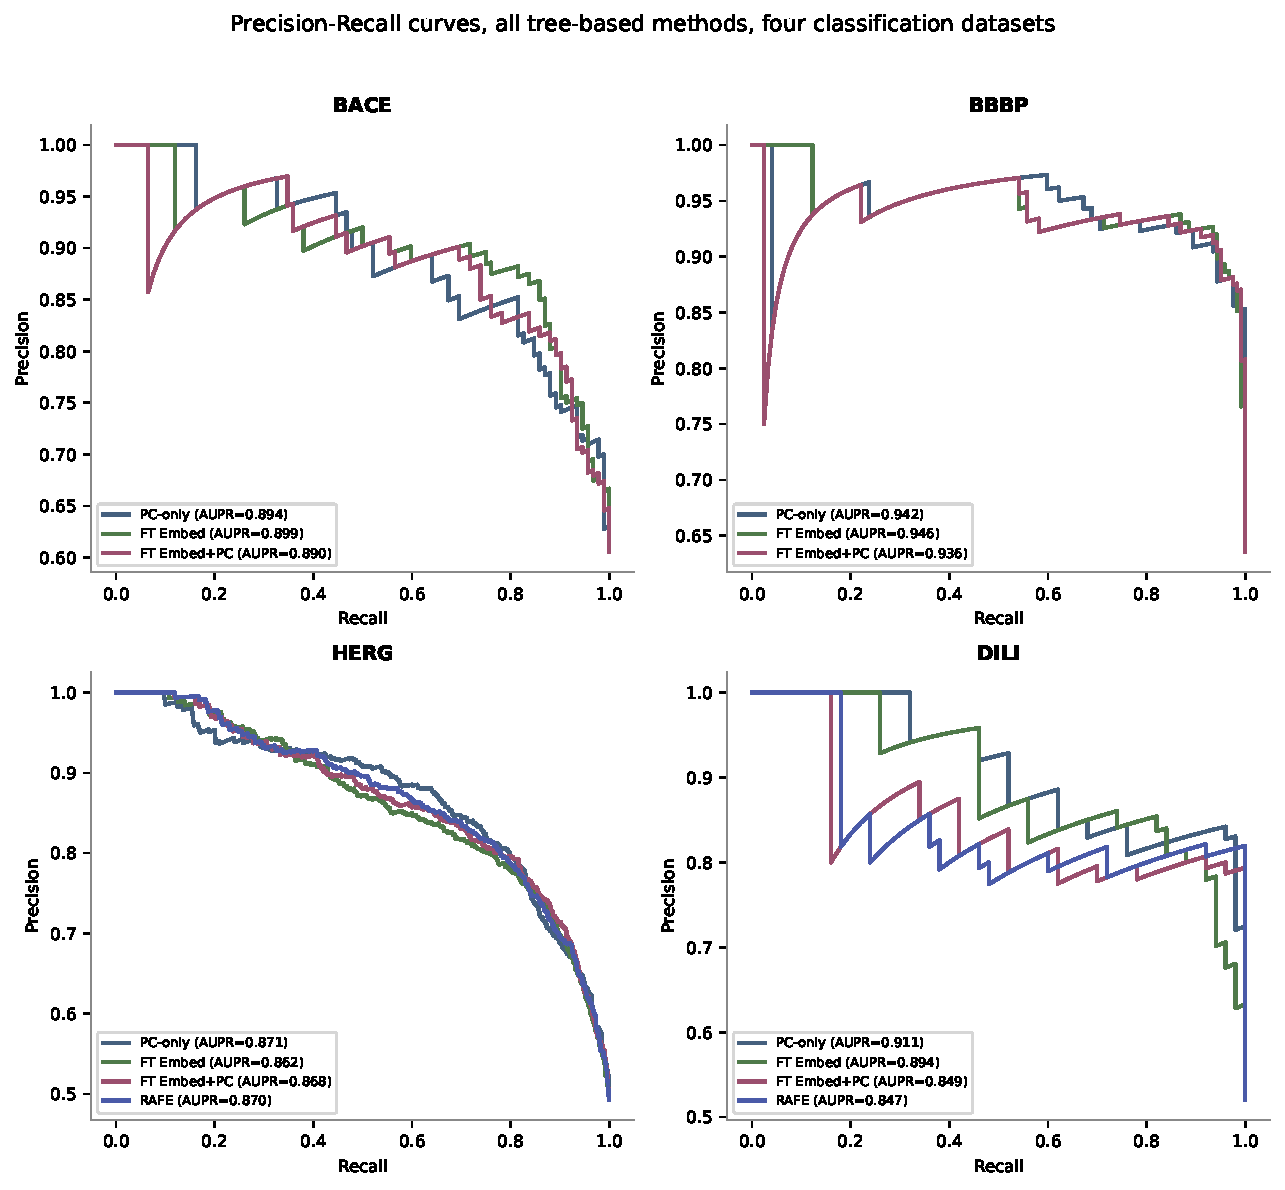
\includegraphics[width=0.95\textwidth]{Figures_v2/pr_curves_4datasets.pdf}
  \caption{Precision-recall curves for the same models and datasets as Figure~\ref{fig:roc_4ds}. DILI's small test set ($n=96$) produces visibly noisier curves than the other three datasets, consistent with its wide bootstrapped SE throughout this paper.}
  \label{fig:pr_4ds}
\end{figure*}

\paragraph{Caco-2 Permeability (Regression).} Table~\ref{tab:caco2} shows the results on the Caco-2 dataset, ranked by Spearman correlation. \textbf{PC-only is the overall winner} (Spearman$=0.853$, R\textsuperscript{2}$=0.744$, SE$=0.021$), ahead of RAFE (ChemBERTa-MTR + CatBoost, Spearman$=0.835$, R\textsuperscript{2}$=0.663$, SE$=0.026$) and FT~Embed+PC (Spearman$=0.824$, R\textsuperscript{2}$=0.672$). Every CLM-based method's band overlaps PC-only's at $\pm1$~SE. This is the clearest example of a task where a purely engineered physicochemical feature set (i.e.\ logP-adjacent descriptors, mechanistically close to membrane permeability) outperforms every CLM-based representation, echoing the pattern already documented for Flavor. A full set of ablation results is available in Supplementary Table~S7.

\begin{table*}[!ht]
\centering
\caption{Best configurations on Caco-2 permeability (regression, TDC ADMET Group), ranked by Spearman.}
\label{tab:caco2}
\begin{adjustbox}{max width=\textwidth}
\begin{tabular}{lllrrrr}
\toprule
Modality & CLM & ML & R\textsuperscript{2} & MAE & Spearman & SE(Spearman) \\
\midrule
PC-only$^*$ & --- & CatBoost & 0.744 & 0.273 & \textbf{0.853} & \textbf{0.0211} \\
Chemprop    & --- & --- & 0.534 & 0.359 & 0.802 & 0.0294 \\
GCN         & --- & --- & 0.244 & 0.491 & 0.733 & 0.0342 \\
\midrule
E2E LoRA    & ChemBERTa-MTR & --- & 0.622 & 0.340 & 0.789 & 0.0318 \\
E2E LoRA    & Uni-Mol       & --- & 0.411 & 0.432 & 0.580 & 0.0565 \\
\midrule
FT Embed    & ChemBERTa-MTR & CatBoost & \textbf{0.668} & 0.318 & 0.821 & 0.0284 \\
FT Embed+PC & ChemBERTa-MTR & LightGBM & 0.672 & \textbf{0.308} & 0.824 & 0.0277 \\
RAFE        & ChemBERTa-MTR & CatBoost & 0.663 & 0.324 & 0.835 & 0.0256 \\
\bottomrule
\end{tabular}
\end{adjustbox}
\end{table*}

\paragraph{Half-Life (Regression).} Table~\ref{tab:half_life} reports results for the Half-Life dataset, again ranked by Spearman correlation. \textbf{FT Embed (MolFormer-XL + XGBoost) is the point-estimate winner} (Spearman$=0.600$, R\textsuperscript{2}$=0.083$, SE$=0.056$), ahead of FT~Embed+PC (Spearman$=0.593$) and PC-only (Spearman$=0.502$, SE$=0.075$). Half-Life is the noisiest dataset in this study ($n_\text{test}=133$, R\textsuperscript{2} $< 0.11$ for every method after log1p transformation and outlier removal); the $\pm1$~SE bands of FT Embed and PC-only overlap substantially, so despite a $+0.098$ Spearman point-estimate gap this is not a confirmed win. Full per-embedding, per-loss ablation is in Supplementary Table~S8.

\begin{table*}[!ht]
\centering
\caption{Best configurations on drug Half-Life (regression, TDC ADMET Group, log1p target), ranked by Spearman.}
\label{tab:half_life}
\begin{adjustbox}{max width=\textwidth}
\begin{tabular}{lllrrrr}
\toprule
Modality & CLM & ML & R\textsuperscript{2} & MAE (h) & Spearman & SE(Spearman) \\
\midrule
PC-only     & --- & XGBoost & 0.110 & 5.687 & 0.502 & 0.0750 \\
Chemprop    & --- & --- & -0.020 & 6.325 & 0.332 & 0.0841 \\
GCN         & --- & --- & 0.114 & 5.928 & 0.418 & 0.0777 \\
\midrule
E2E LoRA    & ChemBERTa-MTR & --- & 0.072 & 6.367 & 0.541 & 0.0654 \\
E2E LoRA    & Uni-Mol       & --- & -0.072 & 6.937 & 0.518 & 0.0720 \\
\midrule
FT Embed$^*$& MolFormer-XL & XGBoost & \textbf{0.083} & \textbf{5.639} & \textbf{0.600} & \textbf{0.0562} \\
FT Embed+PC & MolFormer-XL & XGBoost & 0.090 & 5.594 & 0.593 & 0.0535 \\
RAFE        & MolFormer-XL & XGBoost & 0.090 & 5.557 & 0.568 & 0.0579 \\
\bottomrule
\end{tabular}
\end{adjustbox}
\end{table*}

\subsection{Effectiveness of RAFE: Does Retrieval Substitute for 3D Geometry?}\label{sec:rafe_effectiveness}
RAFE is the point-estimate winner on BBBP (MCC$=0.798$) and DILI (MCC$=0.790$), and competitive with E2E LoRA and FT Embed+PC elsewhere. Its gain over PC-only is closest to statistically confirmed on BBBP, where the $\pm1$~SE bands ($0.798\pm0.028$ vs.\ $0.759\pm0.043$) are close to non-overlapping; on DILI, hERG, Caco-2, and Half-Life, RAFE's (or another method's) point-estimate win over PC-only does not survive a $\pm1$~SE overlap test. Figures~\ref{fig:roc_4ds} and~\ref{fig:pr_4ds} (Section~\ref{sec:new_datasets}) further show that RAFE's ranking among the tree-based modalities is itself dataset-dependent: it is the strongest tree-based modality on BBBP but the weakest of the four on BACE.

Read together with Section~\ref{sec:comparison_sequence}, the picture is that RAFE's label-free ZINC-250k neighborhood context is a genuinely useful, orthogonal signal on tasks like BBBP where bulk physicochemical neighborhood properties (e.g.\ logP) are mechanistically related to the endpoint, but it does \emph{not} substitute for explicit 3D structural information on BACE, where only Uni-Mol's SE(3)-equivariant E2E LoRA clears PC-only by a confirmed margin (Section~\ref{sec:bace_discussion}). In other words, RAFE narrows the practical gap between 1D CLMs and 3D-aware models on some tasks, but where binding-affinity is intrinsically a 3D phenomenon, retrieval over label-free 2D/bulk physicochemical statistics cannot recover the geometric inductive bias that Uni-Mol has built in.

\subsection{Efficiency Analysis}\label{sec:efficiency}
Table~\ref{tab:params} reports LoRA hyperparameters and trainable parameter counts illustrating the range of parameter efficiency across five of the seven datasets. ChemBERTa variants (3.4M base parameters) achieve reductions of $76$-$94\%$ depending on rank; MolFormer-XL ($\approx 46$M parameters) achieves $84$-$97\%$ reduction. Uni-Mol (rank $r \in \{4,8,16,32\}$, targeting only \texttt{in\_proj} across 15 attention layers) achieves particularly efficient adaptation, with $<5\%$ trainable parameters for the lowest-rank configurations. hERG (MolFormer-XL, $r=16$) reduces parameters by $93.91\%$, and DILI (ChemBERTa-MTR, $r=64$) by $76.31\%$. Both fall within the same $76$-$97\%$ range observed elsewhere in the table. Full parameter counts for BACE, BBBP and Flavor datasets are in Supplementary Table~S9.

\begin{table}[!ht]
\centering
\caption{Selected LoRA configurations illustrating the range of parameter efficiency. Trainable~\% = 100 $\times$ trainable / (total parameters + trainable).}
\label{tab:params}
\begin{tabular}{llllrrrr}
\toprule
Dataset & Model & $r$ & $\alpha$ & Total & Trainable & Trainable \% & \% Reduction \\
\midrule
BACE   & ChemBERTa-MLM & 4  & 32  & 3.43M & 205K  & 5.66  & 94.34 \\
BACE   & MolFormer-XL  & 64 & 128 & 45.6M & 8.26M & 15.35 & 84.65 \\
BBBP   & ChemBERTa-MLM & 64 & 32  & 3.43M & 1.06M & 23.69 & 76.31 \\
BBBP   & MolFormer-XL  & 32 & 8   & 45.6M & 4.72M & 9.39  & 90.61 \\
Flavor & MolFormer-XL  & 4  & 64  & 45.6M & 1.63M & 3.44  & 96.56 \\
hERG   & MolFormer-XL  & 16 & 64  & 45.6M & 2.95M & 6.09  & 93.91 \\
DILI   & ChemBERTa-MTR & 64 & 128 & 3.43M & 1.06M & 23.69 & 76.31 \\
\bottomrule
\end{tabular}
\end{table}

Parameter efficiency is a design property, not a per-run measurement, so it is reported once here rather than repeated per dataset. Because LoRA reduces trainable parameters without any corresponding loss in accuracy across the seven datasets studied (Sections~\ref{sec:main_results}), the parameter savings in Table~\ref{tab:params} translate directly into lower fine-tuning memory footprint and training cost relative to full-parameter finetuning of the same backbones, at effectively no cost to the reported MCC/Spearman scores.

\subsection{Ablation Studies}\label{sec:ablations}
The primary ablation axis in this study is \emph{compositional}: Section~\ref{sec:comparison_sequence}'s four-mode ladder (E2E LoRA $\rightarrow$ FT Embed $\rightarrow$ FT Embed+PC $\rightarrow$ RAFE) is itself an ablation over which representational components (end-to-end gradient flow, physicochemical descriptors, ZINC-250k retrieval) are active, and the per-dataset tables in Section~\ref{sec:main_results} report each mode's best CLM/loss/tree-model configuration. A second ablation axis is over \emph{CLM family and finetuning loss}: for every dataset, all CLM variants (ChemBERTa-MLM, ChemBERTa-MTR, MolFormer, Uni-Mol) crossed with all applicable loss functions (WL/FL for classification, Huber for regression) and all three tree-model families are evaluated, with the full per-embedding, per-loss results reported in Supplementary Tables~S2-S9.

Two RAFE-specific hyperparameters -- the number of retrieved neighbors $k$ and the retrieval distance metric -- were fixed by design across all seven datasets rather than swept as an ablation in this study: $k \in \{10, 20\}$ (both used jointly within the same RAFE feature vector, Section~\ref{sec:feature_extraction}) and cosine similarity (via FAISS \texttt{IndexFlatIP} on L2-normalized embeddings) were chosen based on standard retrieval-augmentation practice rather than tuned per dataset. We report this explicitly rather than presenting an ablation that was not run; a systematic sweep over $k$ and alternative distance metrics (e.g.\ Euclidean, Tanimoto-only retrieval) is identified as a concrete direction for future work in Section~\ref{sec:future_work}.

\subsection{Comparison with External Baselines}\label{sec:external_comparison}
Table~\ref{tab:external_main} compares the best PEARL configurations against published graph-based and language-model baselines on BACE, BBBP, and Flavor -- the three MoleculeNet-era datasets for which comparable external LoRA/GNN literature numbers exist. AUC is the primary comparison metric as it is most consistently reported across sources; full method descriptions are in Supplementary Section~S5. The four TDC ADMET datasets have no directly comparable published LoRA baseline, so for those datasets PC-only, Chemprop, and GCN, all run in-house on the identical split, serve as the reference comparison (Section~\ref{sec:new_datasets}).

\begin{table*}[!ht]
\centering
\caption{AUC comparison with published external baselines on MoleculeNet scaffold splits (BACE/BBBP/Flavor only). \textsuperscript{a}~Mean~$\pm$~std over multiple seeds (cited source). \textsuperscript{b}~PEARL point estimate. ``-''~= not reported.}
\label{tab:external_main}
\begin{adjustbox}{max width=\columnwidth}
\begin{tabular}{llccc}
\toprule
\textbf{Method} & \textbf{Ref.} & \textbf{BACE} & \textbf{BBBP} & \textbf{Flavor} \\
\midrule
\multicolumn{5}{l}{\textit{Graph neural network baselines (published)}} \\[2pt]
Chemprop (D-MPNN)      & \cite{yang2019chemprop}  & $0.861 \pm 0.034$\textsuperscript{a} & $0.919 \pm 0.026$\textsuperscript{a} & --- \\
GROVER-Large           & \cite{rong2020grover}    & $0.894 \pm 0.028$\textsuperscript{a} & $0.940 \pm 0.016$\textsuperscript{a} & --- \\
Mole-BERT              & \cite{xia2023molecbert}  & $0.856 \pm 0.029$\textsuperscript{a} & $0.940 \pm 0.011$\textsuperscript{a} & --- \\
\midrule
\multicolumn{5}{l}{\textit{Graph neural network baselines (this work, in-house)}} \\[2pt]
Chemprop    & this work & $0.855$\textsuperscript{b} & $0.918$\textsuperscript{b} & $0.974$\textsuperscript{b} \\
GCN (in-house)         & this work & $0.795$\textsuperscript{b} & $0.924$\textsuperscript{b} & $0.973$\textsuperscript{b} \\
\midrule
\multicolumn{5}{l}{\textit{Chemical language models (full finetuning, published)}} \\[2pt]
Uni-Mol (full FT)      & \cite{zhou2023unimol}    & $0.857 \pm 0.002$\textsuperscript{a} & $0.932 \pm 0.003$\textsuperscript{a} & --- \\
MolFormer-XL (full FT) & \cite{ross2022molformer} & ---                                  & $0.932$\textsuperscript{a}           & --- \\
FART model             & \cite{zimmermann2024fart}& ---                                  & ---                                  & $0.964$ \\
\midrule
\multicolumn{5}{l}{\textit{PEARL (this work, LoRA finetuning)}} \\[2pt]
PEARL Uni-Mol WL (E2E LoRA)   & this work & $\mathbf{0.891}$\textsuperscript{b} & $0.943$\textsuperscript{b}          & $0.973$\textsuperscript{b} \\
PEARL MolFormer FL (E2E LoRA) & this work & $0.872$\textsuperscript{b}          & $0.929$\textsuperscript{b} & $\mathbf{0.975}$\textsuperscript{b} \\
PEARL RAFE best               & this work & $0.858$\textsuperscript{b}          & $\mathbf{0.940}$\textsuperscript{b}          & $0.963$\textsuperscript{b} \\
\midrule
\multicolumn{5}{l}{\textit{PC-only (this work, no CLM)}} \\[2pt]
PC-only (in-house)     & this work & $0.850$\textsuperscript{b}          & $0.937$\textsuperscript{b}          & $0.972$\textsuperscript{b} \\
\bottomrule
\end{tabular}
\end{adjustbox}
\end{table*}

On \textbf{BACE}, PEARL Uni-Mol WL (AUC~$=0.891$) is competitive with GROVER-Large ($0.894\pm0.028$) within the reported standard deviation, and surpasses both the published Uni-Mol full-finetuning result ($0.857$) and the in-house Chemprop/GCN baselines ($\le0.855$). On \textbf{BBBP}, PEARL MolFormer E2E LoRA (AUC~$=0.929$) and RAFE (AUC$=0.940$) both exceed the in-house GCN (AUC$=0.924$) and Chemprop (AUC$=0.918$) baselines, and RAFE exceeds GROVER-Large and Mole-BERT (both $0.940$, tied). On \textbf{Flavor}, in-house Chemprop (AUC$=0.974$) is essentially tied with PEARL MolFormer E2E LoRA ($0.975$): the CLM ladder's margin over a graph-only baseline is negligible on this dataset, consistent with the PC-only finding in Section~\ref{sec:comparison_sequence}.

\subsection{Discussion}\label{sec:bace_discussion}
Across seven datasets and two task types (classification, regression), PEARL pushes parameter-efficient molecular property prediction forward while holding every claimed improvement to an in-house, identically-evaluated GNN and PC-only baseline suite, rather than leaning on numbers borrowed from other papers.

\textbf{3D geometry matters for binding-affinity tasks:} Uni-Mol's SE(3)-equivariant architecture provides the most accurate BACE inhibitor classification (MCC$=0.623$, SE$=0.039$), an 8\% absolute gain over the best SMILES-based method and the only result where the CLM ladder's $\pm1$~SE band does not overlap PC-only's. BACE-1 inhibitor activity is governed by three-dimensional ligand-receptor complementarity, and the inductive biases of a geometry-aware transformer are well-matched to this task.

\textbf{PC-only remains a strong, hard-to-beat baseline.} Across all seven datasets studied here, PC-only alone (473 engineered physicochemical descriptors, no CLM, no LoRA, no retrieval) wins outright on Caco-2 (Spearman$=0.853$) and is statistically indistinguishable at $\pm1$~SE from the best CLM-based method on Flavor, hERG, and Half-Life. Only on BACE does a CLM-based method (Uni-Mol E2E LoRA) clear PC-only by a margin that survives the $\pm1$~SE screen; on BBBP and DILI, RAFE's point-estimate lead over PC-only is directionally favorable but does not reach that same bar. We report this transparently because it is the central question this benchmark asks: \emph{does the added complexity of CLM finetuning, LoRA adaptation, and retrieval augmentation earn its keep over a simple, fast, fully-interpretable tree ensemble on engineered descriptors?} Dataset by dataset, the answer is: sometimes. And where it clearly does pay off (BACE), the task happens to be mechanistically tied to 3D structure rather than to bulk physicochemical properties.

\textbf{Task-dependent optimal strategies persist:} (i)~MolFormer consistently outperforms ChemBERTa across SMILES-based conditions; (ii)~weighted loss excels on severely imbalanced datasets (BBBP, Flavor, hERG-WL), while focal loss is optimal for DILI and BBBP; (iii)~adding PC features to finetuned embeddings provides minimal improvement over finetuned embeddings alone in most cases, because LoRA adaptation already internalizes task-relevant molecular properties; (iv)~for regression tasks (Caco-2, Half-Life), gains over PC-only are smaller and less consistent than for classification, suggesting CLM embeddings are relatively less informative for these ADMET endpoints than for binding-affinity or permeability-adjacent tasks.

%% =====================================================================
\section{Conclusion and Future Work}\label{sec:conclusion}

PEARL establishes a practical and thoroughly-benchmarked framework for molecular property prediction, combining parameter-efficient 3D and SMILES-based finetuning with retrieval-augmented chemical neighborhood context, evaluated across seven classification and regression datasets against in-house GNN and PC-only baselines. PEARL achieves the best reported result on BACE (Uni-Mol, MCC$=0.623$) and BBBP (RAFE, MCC$=0.798$), while transparently reporting that on Flavor, hERG, Caco-2, and Half-Life the simpler PC-only baseline remains statistically competitive, all while reducing trainable parameters by $76$-$97\%$.

\subsection{Limitations}\label{sec:limitations}
Several limitations bound how these results should be read. First, RAFE's benefit is retrieval-density dependent: because ZINC-250k is a drug-like, general-purpose corpus, a query molecule with few close chemical neighbors in ZINC-250k (e.g.\ a highly novel scaffold, or a molecule from a chemical class underrepresented in ZINC-250k, such as some DILI or hERG actives) is likely to receive a less informative RAFE feature vector than one embedded in a dense region of the retrieval corpus; we did not stratify results by neighbor density in this study. Second, several test sets are small (DILI $n=96$; Caco-2 $n=182$; Half-Life $n=133$; BACE $n\approx152$), which widens bootstrapped confidence intervals and limits our ability to statistically confirm point-estimate wins even where the margin is largest (DILI). Third, as noted in Section~\ref{sec:ablations}, the number of retrieved neighbors $k$ and the retrieval distance metric were fixed by design rather than tuned per dataset, so the reported RAFE results represent one reasonable configuration rather than an optimum found via a dedicated sweep.

\subsection{Future Directions}\label{sec:future_work}
A systematic ablation over the RAFE hyperparameters identified in Section~\ref{sec:ablations} -- the number of retrieved neighbors $k$ and the choice of retrieval distance metric (e.g.\ Euclidean distance, or fingerprint-only Tanimoto retrieval in place of embedding cosine similarity) -- would clarify how sensitive RAFE's gains are to these design choices, and whether per-dataset tuning could close more of the gap to explicit 3D geometry on structure-governed tasks. Extending PEARL's regression support with calibrated uncertainty estimates (e.g., quantile regression or conformal prediction on top of the tree-based stage) would make the Caco-2/Half-Life results more directly actionable for prioritization decisions. Emerging multi-modal CLMs such as nach0~\cite{livne2024nach0} and Omni-Mol~\cite{hu2025omnimol} represent natural extensions of the LoRA + RAFE paradigm, and expanding PEARL to multimodal graph-text foundation models is a promising direction for capturing structural and textual context jointly. Finally, given how consistently PC-only competes with the full CLM ladder in this study, future benchmarking of molecular CLMs should treat a PC-only baseline as a mandatory control, not an optional ablation.

%% =====================================================================
\section*{Declarations}

\noindent\textbf{Funding.} This research did not receive any specific grant from funding agencies in the public, commercial, or not-for-profit sectors.

\noindent\textbf{Competing interests.} The authors declare no competing financial interests. R.M.\ is Scientific Advisor at Eternal, U.A.E.

\noindent\textbf{Data availability.} All code and data associated with PEARL, including the TDC data-curation, RAFE, and in-house GNN baseline pipelines, is available at \url{https://github.com/raghvendra5688/PEARL}.

\noindent\textbf{Acknowledgments.} We thank the Qatar National Library (QNL) for their support in providing resources and funding the APC.

\noindent\textbf{Author contributions.} K.A. contributed to Methods, Experiments, Validation, Writing -- original draft. S.G. and H.B. participated in Project Supervision, Writing -- review \& editing. R.M. conceptualized and supervised the project, and contributed to Methods, Experiments, Validation, Writing -- review \& editing.

\section*{Supplementary information}
The supplementary material accompanying this article contains additional experimental details, complete ablation studies, feature descriptions, and implementation details supporting the results presented in the main manuscript (Supplementary Tables S1-S9; Supplementary Sections S1-S5).

\bibliographystyle{unsrt}
\bibliography{sn-bibliography}

\end{document}
